% ILS
% version 2023
%-------------------------------------------------------

% 2023viii21 revisar el siguiente link
% https://simpleflying.com/approach-types-guide/

\subsection{Introducción}
\label{06.01.introduccion}

Los sistemas de aproximación de aterrizaje son aquellos que proporcionan una guía al piloto de
una aeronave que desciente, para facilitarle la aproximación y aterrizaje a la pista del aeropuerto que
desea. Estos están normalizados según el tipo de pista, la OACI distingue entre:

\begin{itemize}
\item Pista de vuelo visual y
\item Pista de vuelo por instrumentos o Pista para aproximaciones de precisión
\end{itemize}

Se debe diferenciar entre aproximación y aterrizaje.

\begin{description}
\item [Aproximación:] consiste en una fase
de vuelo que comienza en el momento que se deja el vuelo de crucero para iniciar la maniobra de
acercamiento con descenso y finaliza en el momento en que se llega al punto de decisión, definido
como aquel en que se debe determinar si se aterriza o se frustra la maniobra, para elevarse de nuevo.

\item[Aterrizaje:]  es la operación que empieza en el punto de decisión, cuando ya se ha
  decidido tomar tierra y no se puede frustrar el aterrizaje, finalizando cuando la aeronave
  se ha posado en la pista, disminuyendo su velocidad hasta el punto de no poder abandonarla.
\end{description}

Una aproximación correcta conduce a un aterrizaje exitoso, por lo que son interdependientes uno
del otro.

La maniobra de aproximación suele dividirse en tres fases:

\begin{description}
\item [Aproximación inicial:] establece la transición entre vuelo de
  crucero y configuración de descenso. Se modifican los parámetros
  de velocidad y altura a la aproximación, los sistemas de navegación
  empleados son VOR, TACAN o ADF. Desde el control de tierra se puede
  ordenar modificar la trayectoria.
  
\item [Aproximación intermedia:] se
  siguen empleando los sistemas de navegación en el crucero, per la
  altitud, velocidad y distancia de separación con otras aeronaves
  cobran una relevancia especial. Esta fase termina en el punto en que
  se puede empezar a emplear el sistema de navegación de aproximación
  (PAR, ILS y MLS) con seguridad.
  
\item [Aproximación final:] en esta fase la
  aeronave ha interceptdo los haces del sistema de aproximación y
  está prácticamente alineada con la pista. La fase finaliza con el
  avión, ya posado en la pista, se encuentra con velocidad segura para
  abandonarla.
\end{description}

Para el caso del uso de instrumentos para la aproximación la OACI establece un procedimiento respectivo.


Los distintos sistemas disponibles para estas maniobras pueden ser clasificados según la forma de transmitir la información:

\begin{itemize}
\item Ayudas visuales
  \begin{itemize}
  \item Sistemas de Luces de Aproximación
  \item Sistema  Indicador de Pendiente de Aproximación Visual
  \item Indicador de Trayectoria de Aproximación de Precisión
  \end{itemize}
\item Ayudas radioeléctricas
\end{itemize}

\begin{figure}[!h]
  \centering
  
\includegraphics[width = 0.8\textwidth]{06.radionavegacion/Imagenes/06.Sistemas.Aproximacion/shutterstock_592939535.jpg}
  \caption{Aproximación a pista de un Boeing 767. Fuente: Aureliy I Shutterstock }
  \label{fig:06.sistemas.aproximacion.pista}
\end{figure}



\subsection{Requerimientos normativos}
\label{sec:06.requerimientos.normativos.aproximacion}


\begin{tcolorbox}[title={
    OACI. Anexo 14. Edición 2018
  }
  ]
  {\footnotesize
   {\bf  Pista de vuelo visual :} 
    Pista destinada a las operaciones de aeronaves que utilicen procedimientos de aproximación visual
    o un procedimiento de aproximación por instrumentos a un punto más allá del cual pueda continuarse
    la aproximación en condiciones meteorológicas de vuelo visual.

\emph{Nota. Las condiciones meteorológicas de vuelo visual (VMC) se describen en el Capítulo 3 del Anexo 2 — Reglamento
del aire.
}

{\bf Pista de vuelo por instrumentos o Pista para aproximaciones de precisión:} 
   Uno de los siguientes tipos de pista destinados a la operación de aeronaves que utilizan
    procedimientos de aproximación por instrumentos:
    
    \begin{enumerate}[a)]
    \item Pista para aproximaciones que no son de precisión. Pista de vuelo servida por ayudas visuales y ayudas no visuales
destinada a operaciones de aterrizaje después de una operación de aproximación por instrumentos de Tipo A y con
visibilidad no inferior a 1000 m.
\item Pista para aproximaciones de precisión de Categoría I. Pista de vuelo servida por ayudas visuales y ayudas no
visuales destinadas a operaciones de aterrizaje después de una operación de aproximación por instrumentos de Tipo B
con una altura de decisión (DH) no inferior a 60 m (200 ft) y con una visibilidad de no menos de 800 m o con un
alcance visual en la pista no inferior a 550 m.
\item Pista para aproximaciones de precisión de Categoría II. Pista de vuelo servida por ayudas visuales y ayudas no
visuales destinadas a operaciones de aterrizaje después de una operación de aproximación por instrumentos de Tipo B
con una altura de decisión (DH) inferior a 60 m (200 ft) pero no inferior a 30 m (100 ft) y con un alcance visual en la
pista no inferior a 300 m.
\item Pista para aproximaciones de precisión de Categoría III. Pista de vuelo servida por ayudas visuales y ayudas no
visuales destinada a operaciones de aterrizaje después de una operación de aproximación por instrumentos de Tipo B
hasta la superficie de la pista y a lo largo de la misma; y

\begin{enumerate}[A ]
\item Destinada a operaciones con una altura de decisión (DH) inferior a 30 m (100 ft), o sin altura de decisión y un
alcance visual en la pista no inferior a 175 m.
\item Destinada a operaciones con una altura de decisión (DH) inferior a 15 m (50 ft), o sin altura de decisión, y un
alcance visual en la pista inferior a 175 m pero no inferior a 50 m.
\item Destinada a operaciones sin altura de decisión (DH) y sin restricciones de alcance visual en la pista.
\end{enumerate}

\end{enumerate}

\emph{Nota 1. Las ayudas visuales no tienen necesariamente que acomodarse a la escala que caracterice las ayudas no visuales que se proporcionen. El criterio para la selección de las ayudas visuales se basa en las condiciones en que se trata de operar. \\
Nota 2. Consúltese el Anexo 6,  Operación de aeronaves, para los tipos de operaciones de aproximación por
instrumentos.
}


  }
  
\end{tcolorbox}

\begin{tcolorbox}[title={Procedimiento de aproximación por instrumentos (IAP). OACI Anexo 6. Edición 2018}]
  {\footnotesize

    Serie de maniobras predeterminadas realizadas por referencia a los instrumentos de a bordo, con protección específica contra los obstáculos desde el punto de referencia de aproximación inicial, o, cuando sea el caso, desde el inicio de una ruta definida de llegada hasta un punto a partir del cual sea posible hacer el aterrizaje; y, luego, si no se realiza éste, hasta una posición en la cual se apliquen los criterios de circuito de espera o de margen de franqueamiento de obstáculos en ruta. Los procedimientos de aproximación por instrumentos se clasifican como sigue:
    
    \begin{description}
    \item [Procedimiento de aproximación que no es de precisión, \ac{NPA}]. Procedimiento de aproximación por instrumentos diseñado para operaciones de aproximación por instrumentos 2D de Tipo A.

\emph{Nota. Los procedimientos de aproximación que no son de precisión pueden ejecutarse aplicando la técnica de
Aproximación Final en Descenso Continuo, \ac{CDFA}. Las \ac{CDFA} con guía \ac{VNAV} de asesoramiento, calculada por el equipo de
a bordo se consideran operaciones de aproximación por instrumentos 3D. Las \ac{CDFA} con cálculo manual de la velocidad
vertical de descenso requerida se consideran operaciones de aproximación por instrumentos 2D. En los PANS-OPS
(Doc 8168), Volumen I, Parte II, Sección 5, se proporciona más información sobre las CDFA.
}

\item [Procedimiento de aproximación con guía vertical (APV)]. Procedimiento de aproximación por instrumentos, con
navegación basada en la performance (PBN), diseñado para operaciones de aproximación por instrumentos 3D de
Tipo A.

\item[ Procedimiento de aproximación de precisión (PA)]. Procedimiento de aproximación por instrumentos, basado en sistemas
de navegación (ILS, MLS, GLS, y SBAS CAT I), diseñado para operaciones de aproximación por instrumentos 3D de
Tipo A o B.

\emph{Nota. Véase 4.2.8.3 en relación con los tipos de operaciones de aproximación por instrumentos.
}

\end{description}
  }
\end{tcolorbox}

\begin{tcolorbox}
  {\footnotesize

    \begin{description}
      
\item[4.2.8.3] Las operaciones de aproximación por instrumentos se clasificarán basándose en los mínimos de utilización más
bajos por debajo de los cuales la operación de aproximación deberá continuarse únicamente con la referencia visual requerida,
de la manera siguiente:

\begin{enumerate}[a)]
\item \textbf{Tipo A:} una altura mínima de descenso o altura de decisión igual o superior a 75 m (250 ft); y
\item \textbf{Tipo B:} una altura de decisión inferior a 75 m (250 ft). Las operaciones de aproximación por instrumentos de Tipo B están categorizadas de la siguiente manera:
  \begin{enumerate}[1)]
  \item  \textbf{Categoría I (CAT I):} una altura de decisión no inferior a
    60 m (200 ft) y con visibilidad no inferior a 800 m o alcance
    visual en la pista no inferior a 550 m; 
  \item \textbf{Categoría II (CAT II):}
    una altura de decisión inferior a 60 m (200 ft), pero no inferior
    a 30 m (100 ft) y alcance visual en la pista no inferior a 300 m;
    
  \item \textbf{Categoría IIIA (CAT IIIA):} una altura de decisión inferior a 30
    m (100 ft) o sin limitación de altura de decisión y alcance visual
    en la pista no inferior a 175 m; 
  \item \textbf{Categoría IIIB (CAT IIIB):} una
    altura de decisión inferior a 15 m (50 ft) o sin limitación de
    altura de decisión y alcance visual en la pista inferior a 175 m
    pero no inferior a 50 m; y 
  \item \textbf{Categoría IIIC (CAT IIIC):} sin
    altura de decisión ni limitaciones de alcance visual en la pista.
\end{enumerate}

\end{enumerate}

\emph{Nota 1. Cuando los valores de la altura de decisión (DH) y del alcance visual en la pista (RVR) corresponden a
categorías de operación diferentes, la operación de aproximación por instrumentos ha de efectuarse de acuerdo con los
requisitos de la categoría más exigente (p. ej., una operación con una DH correspondiente a la CAT IIIA, pero con un RVR de
la CAT IIIB, se consideraría operación de la CAT IIIB, o una operación con una DH correspondiente a la CAT II, pero con un
RVR de la CAT I, se consideraría operación de la CAT II).\\
Nota 2. La referencia visual requerida significa aquella sección de las ayudas visuales o del área de aproximación que
debería haber estado a la vista durante tiempo suficiente para que el piloto pudiera hacer una evaluación de la posición y de la rapidez del cambio de posición de la aeronave, en relación con la trayectoria de vuelo deseada. En el caso de una operación de aproximación en circuito, la referencia visual requerida es el entorno de la pista.
}

\end{description}
}
\end{tcolorbox}



\begin{figure}[!htb]
  \centering
  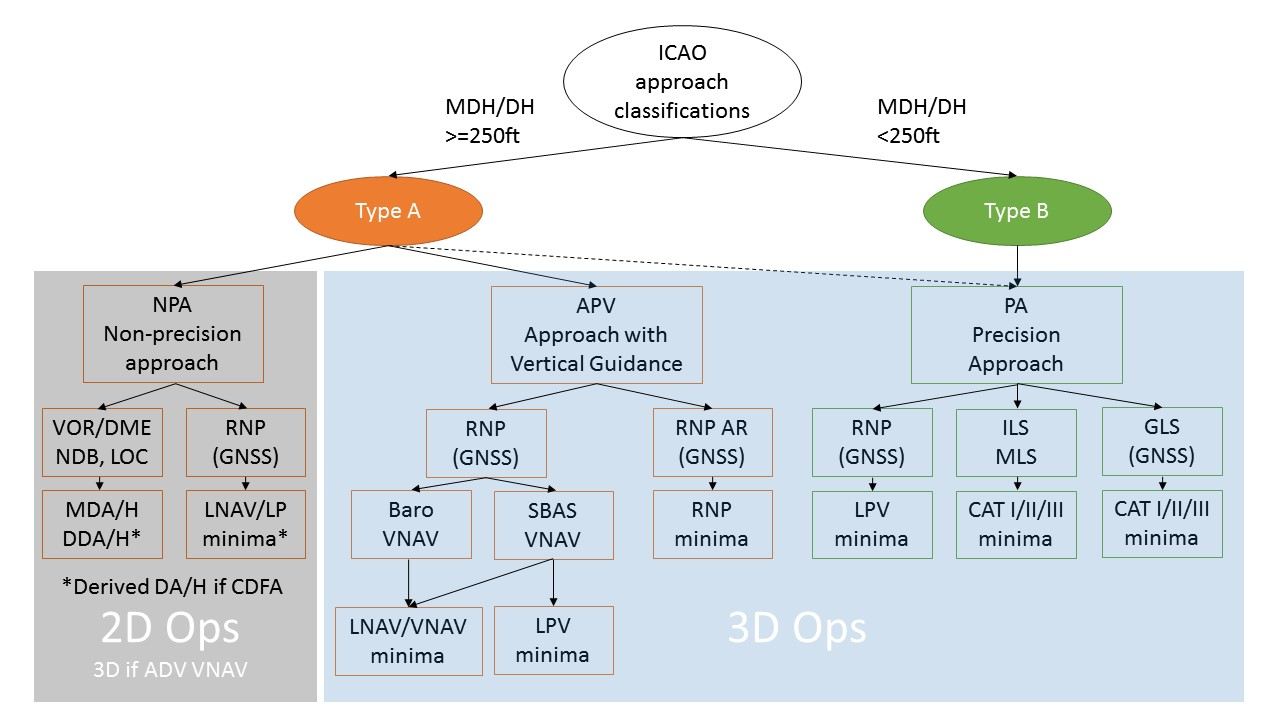
\includegraphics[width=0.9\textwidth]{06.radionavegacion/Imagenes/OACI-Doc8168-tiposInstrumentosAproximacion.jpg} 
  \caption{Tipos de instrumentos para aproximación según OACI \protect\cite{NuevasAproximaciones}}
  \label{fig:06.tipos.instrumentos.aproximacion}
\end{figure}


\begin{table}[!htb]
  \centering
  \caption[06.OACI.requisitos.]{OACI Requisitos de performance en apoyo de las operaciones de aproximación por instrumentos}
  \label{tab:06.OACI.requisitos}
{\footnotesize
  \begin{tabular}{lm{0.25\textwidth}m{0.2\textwidth}} \hline 
    \multicolumn{2}{c}{Performance de sistemas en el Anexo 10}
    & {Método del Anexo 6 - Categoría de operación de aproximación}
    \\ \hline 
    Aproximación que no es de precisión (NPA)
    &
    &2D-Tipo A$^1$
    \\ \hline
    Aproximación con guía vertical (APV)
    &
    &3D-Tipo A$^2$
    \\ \hline
    Aproximación de precisión (PA)
    & Categoría I, DH igual o superior a 75 m (250 ft)
    &3D-Tipo A$^3$ \\ \cline{2-3}
    & Categoría I, DH igual o superior a 60 m (200
      ft) e inferior a 75 m (250 ft)
    & 3D-Tipo B - CAT I $^3$ \\ \cline{2-3}
    & Categoría II
    & 3D-Tipo B - CAT II \\ \cline{2-3}
    & Categoría II
    & 3D-Tipo B - CAT II \\  \hline
    \multicolumn{3}{l}{\footnotesize
    \parbox{\linewidth}{
        $^1$ Sin  guía vertical barométrica \\
    $^2$ Con guía vertical barométrica o SBAS \\
    $^3$ Con guía vertical ILS, MLS, GBAS o SBAS.
    }	
    } \\
  \end{tabular}
  }
\end{table}

\href{https://skybrary.aero/sites/default/files/bookshelf/2991.pdf}{OACI Doc 9613
  Performance-Based Navigation Manual}


\subsection{Ayudas visuales}
\label{sec:06.02.ayudasvisuales}


Las ayudas visuales utilizan la energía electromagnética como portadora de información y permiten
realizar con mayor eficacia el contacto visual con la pista de aterrizaje y con la trayectoria
correcta de la senda de descenso.

Son dispositivos luminosos cromáticos que emplean el contraste para
transmitir la información al piloto.

Como es lógico, estas ayudas son indispensables en aterrizajes
nocturnos o diurnos de baja visibilidad.

En cuanto a las características que las ayudas visuales  presentan son  descritas
por lo que se denomina las ``\emph{5C}'': 

\begin{description}
  
\item [Configuración] se refiere a la forma de emplazamiento de las
unidades que componen cualquier sistema de ayuda visual iluminada, especificando distancias
entre ellas, distancias respecto al umbral de pista (sector desde donde se inicia el área destinada a
las operaciones aéreas), etc.

\item[Color] los colores según norma utilizados para diferenciar las señales de las ayudas visuales iluminadas.

\item[Cobertura] se refiere a los sectores en los que son visibles las ayudas visuales iluminadas y a la reducción del
  deslumbramiento.
  
\item[Candelas] unidad de intensidad lumínica, las recomendaciones que la OACI emite son
curvas de isocandelas las cuales deben cumplirse y que varía de acuerdo a la posición y función
de las ayudas visuales iluminadas (diagramas publicados en el Anexo 14).

Se sabe que la agudeza visual y la sensibilidad frente al deslumbramiento varían según las
personas, la edad de ellas y el grado de fatiga.  Un elemento importante para el deslumbramiento
es la transmitibilidad atmosférica, que varía cuando es de día, atardecer, noche o cuando
existe niebla.

Para otorgar un buen servicio, dentro las operaciones aéreas, a los pilotos evitando los
problemas de deslumbramiento, los reguladores de corriente constante poseen un rango de
variación de intensidad lumínica (variación de brillo) que depende de las características de las
ayudas visuales.

Por lo general las luces de alta y media intensidad posee de 3 a 5 niveles de intensidad, en cambio
las luces de baja intensidad solo posee un solo nivel de intensidad.

\item[Continuidad] las ayudas visuales más críticas deben tener un alto grado de continuidad en la
emisión de sus señales, por lo que se tienen dos circuitos eléctricos en las luces de borde de pista
y luces de aproximación, en caso de falla de uno de ellos el otro se mantiene operable y aun son
visibles las señales luminosas.

\end{description}




\subsubsection{Sistemas de Luces de Aproximación}
\label{sec:06.02.01.ALS}

El Sistema de Luces de Aproximación (ALS,  Approach Light Systems) se utiliza en aeródromos
con alta frecuencia de uso. Se ubican en las cercanias de la cabecera de la pista como parte a las
ayudas electrónicas de navegación para la parte final de aproximaciones precisas y no precisas de un
vuelo IFR, y también como una guía visual en vuelos VFR nocturnos.
En la Figura \ref{fig:06.ALS.aeropuerto} puede observarse el ALS de la aproximación a la pista 27
del aeropuerto Liverpool - John Lennon.

El ALS suministra al piloto con entradas visuales respecto a la alineación de la aeronave, el
balance, el horizonte, el ancho y la posición con respecto a la cabecera de la pista. Desde que los
sistemas de iluminación aeroportuarios relevaron a las necesariamente rápidas acciones mentales
sobre la información visual que encabezaban las decisiones, un sistema visual es ideal para una guía
durante los últimos segundos críticos del movimiento descendente sobre el patrón de planeo.

El sistema de luces de aproximación se creó en base al ángulo del patrón de planeo, el rango visual,
el ángulo de visibilidad cortada en la cabina y de las velocidades de aterrizaje. Esto es esencial para
que los pilotos estén propensos a utilizar e identificar ALS y de interpretar el sistema sin confusión.
El sistema comienza en el umbral de cabecera de pista y se extiende hacia el frente de la misma por,
aproximadamente, 900 m (3000 pies). En caso de que esta longitud no pueda ser utilizada, se emplea
la mayor posible. Una columna de luces estroboscópicas de alta intensidad luminosa, alimentadas
mediante una descarga de condensador e igulamente espaciadas, se coloca alineada con el eje de la
pista y al ser accionadas producen un efecto de flash que indica a los pilotos la ubicación del centro
de la pista en condiciones de baja visibilidad.

En los Estados Unidos de América los ALS poseen una Fila de Decisión (Decision Bar), ubicada
a 1000 pies (300 m) de la cabecera de pista, la cual sirve como un horizonte visible para facilitar
la transición de IFR a VFR. También se la ubica de forma que coincida con la Altura de Decisión
(Decision Altitude).

\begin{tcolorbox}[title={Requerimientos OACI. Anexo 14. Volumen I. Edición 2018.
    }]
{\footnotesize
  \begin{description}
  \item [5.3.4.1]  Aplicación
    \begin{enumerate}[A ]
    \item {\bf Pista de vuelo visual}
      
      Recomendación. Cuando sea materialmente posible, debería instalarse un sistema sencillo de iluminación de aproximación tal como el que se especifica en 5.3.4.2 a 5.3.4.9, para servir a una pista de vuelo visual cuando el número de clave sea 3 ó 4 y destinada a ser utilizada de noche, salvo cuando la pista se utilice solamente en condiciones de buena visibilidad y se proporcione guía suficiente por medio de otras ayudas visuales.
      
{\it Nota. También puede instalarse un sistema sencillo de iluminación de aproximación para proporcionar guía visual
  durante el día.}

\item {\bf  Pista para aproximaciones que no son de precisión}
  
Cuando sea materialmente posible, se instalará un sistema sencillo de iluminación de aproximación, tal como el que se
especifica en 5.3.4.2 a 5.3.4.9, para servir a una pista para aproximaciones que no son de precisión, salvo cuando la pista se
utilice solamente en condiciones de buena visibilidad y se proporcione guía suficiente por medio de otras ayudas visuales.

\emph{Nota. Es conveniente que se considere la posibilidad de instalar un sistema de iluminación de aproximación de
precisión, de Categoría I, o la adición de un indicador que lleve a la pista.}

\item \textbf{ Pista para aproximaciones de precisión de Categoría I}
  
Cuando sea materialmente posible, en una pista para aproximaciones de precisión de Categoría I se instalará un sistema de
iluminación de aproximación de precisión de Categoría I, tal como el que se especifica en 5.3.4.10 a 5.3.4.21.

\item \textbf{ Pista para aproximaciones de precisión de Categorías II y III}
  
En una pista para aproximaciones de precisión de Categorías II y III, se instalará un sistema de iluminación de
aproximación de precisión de las Categorías II o III, tal como se especifica en 5.3.4.22 a 5.3.4.39.


\end{enumerate}
\end{description}
}
\end{tcolorbox}




Diversas configuraciones de ALS son reconocidas por la OACI, sin embargo, configuraciones no
normalizadas se encuentran instaladas en diversos aeropuertos. Los ALS son sistemas de luces de alta
intensidad y varios se complementan con otros ubicados sobre la senda de aproximación, tal como el
Runway End Identifier Lights (REIL), Touchdown Zone Lights (TDZL), and High Intensity Runway
Lights (HIRL). Entre las configuraciones más usuales se tienen:

{\footnotesize
\begin{description}
\item[MALSR:] Medium-intensity Approach
Lighting System with Runway Alignment
Indicator Lights

\item[MALSF:] Medium-intensity Approach
Lighting System with Sequenced Flashing
lights

\item[SALS:] Simple Approach Lighting System

\item[SSALS:] Simplified Short Approach Lighting System

\item[SSALR:] Simplified Short Approach Light-
ing System with Runway Alignment Indicator Lights

\item[ODALS:] Omnidirectional Approach Lighting System
  
\item[ALSF-1:] Approach Lighting System with
  Sequenced Flashing Lights configuration 1
  
\item[ALSF-2:] Approach Lighting System with
  Sequenced Flashing Lights configuration 2
  
\item[CALVERT I/ICAO-1 HIALS:] ICAO-compliant configuration 1 High Intensity
  Approach Lighting System
  
\item[CALVERT II/ICAO-2 HIALS:] ICAO-compliant configuration 2 High Intensity
  Approach Lighting System
  
\item[LDIN:] Lead-in lighting
  
\item[REIL:] Runway End Identification Lights

\item[RAIL:] Runway Alignment Indicator Lights

\end{description}
}

En las configuraciones que poseen luces secuenciadas (sequenced flashing lights), estas son de tipo
estroboscópicas y se ubican de frente a la cabecera de pista, sobre el eje de la misma. Estas luces
se encienden en secuencia, comenzando con la luz más distante de la cabecera y terminando en la
Fila de Decisión (Decision Bar). Esto se justifica para no distraer al piloto durante la fase crítica de cambiar de IFR a VFR. El sistema de luces secuenciadas es comunmente conocido como ``\emph{el conejo}'' (the rabbit) o ``\emph{correr al conejo}'' (the running rabbit).

\begin{figure}[!htb]
  \centering
  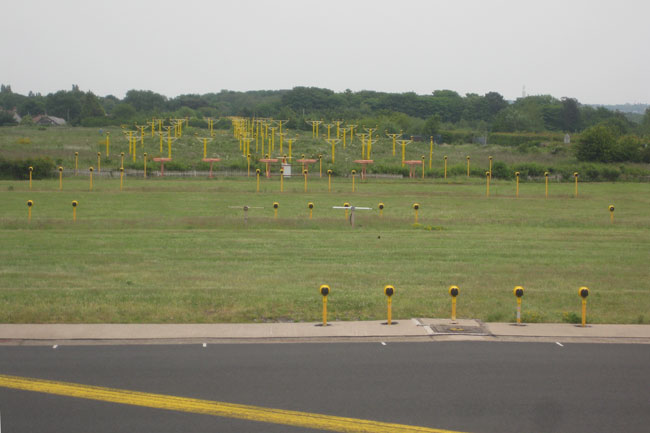
\includegraphics[width=0.7\textwidth]{06.radionavegacion/Imagenes/06.ALS/ALS-01.jpg} 
  \caption{ALS \protect\cite{ALSfoto}}
  \label{fig:06.ALS.aeropuerto}
\end{figure}



\subsubsection{Sistema  Indicador de Pendiente de Aproximación Visual }
\label{sec:06.02.02.VASIS}


\begin{tcolorbox}[title=Requerimientos OACI. Anexo 14. Volumen I. Edición 2018.\\
  5.3.5 Sistemas visuales indicadores de pendiente de aproximación
  ]

  {\footnotesize

    \begin{description}
    \item [5.3.5.1] Se instalará un sistema visual indicador de pendiente de aproximación para facilitar la aproximación a una pista, que cuente o no con otras ayudas para la aproximación, visuales o no visuales, cuando exista una o más de las condiciones
siguientes:
\begin{enumerate}[a)]
\item La pista sea utilizada por turborreactores u otros aviones
  con exigencias semejantes en cuanto a guía para la aproximación; 
\item el piloto de cualquier tipo de avión pueda tener dificultades para
  evaluar la aproximación por una de las razones siguientes:

  \begin{enumerate}[1)]
  \item orientación visual insuficiente, por ejemplo, en una
    aproximación de día sobre agua o terreno desprovisto de puntos de
    referencia visuales o durante la noche, por falta de luces no
    aeronáuticas en el área de aproximación; o 
  \item información visual
    equívoca, debida por ejemplo, a la configuración del terreno
    adyacente o a la pendiente de la pista;
  \end{enumerate}

\end{enumerate}
\end{description}
}
\end{tcolorbox}

\begin{tcolorbox}[title=Requerimientos OACI. Anexo 14. Volumen I. Edición 2018.\\
  5.3.5 Sistemas visuales indicadores de pendiente de aproximación 
  (Continuación)
  ]

  {\footnotesize

    \begin{description}
      
    \item[   ] 
    \begin{enumerate}

       \item la presencia de objetos en el área de aproximación pueda constituir un peligro grave si un avión desciende por debajo de la trayectoria normal de aproximación, especialmente si no se cuenta con una ayuda no visual u otras ayudas visuales que adviertan la existencia de tales objetos;

       \item las características físicas del terreno en cada extremo de la pista constituyan un peligro grave en el caso en que un avión efectúe un aterrizaje demasiado corto o demasiado largo; y

       \item las condiciones del terreno o las condiciones meteorológicas predominantes sean tales que el avión pueda estar sujeto a turbulencia anormal durante la aproximación.
         
\end{enumerate}

\item[5.3.5.2] Los sistemas visuales indicadores de pendiente de aproximación normalizados consistirán en lo siguiente:

  \begin{enumerate}[a)]

  \item  T-VASIS y AT-VASIS que se ajusten a las especificaciones
    contenidas en 5.3.5.7 a 5.3.5.23 inclusive; 

  \item PAPI y APAPI que se
    ajusten a las especificaciones contenidas en 5.3.5.24 a 5.3.5.41
    inclusive; según se indica en la Figura \ref{fig:06.sistemas.indicadores.pendiente.aproximacion}.
    
  \end{enumerate}
  
\item [5.3.5.3] Se instalarán PAPI, T-VASIS o AT-VASIS si el número de clave es 3 ó 4 o cuando existe una o más de las condiciones especificadas en 5.3.5.1.

\item [5.3.5.4 Recomendación.] A partir del 1 de enero de 2020,
    debería discontinuarse el uso de T-VASIS y AT-VASIS como sistemas
    indicadores de pendiente en aproximación visual.
  
    \end{description}
}


\end{tcolorbox}


El Sistema Indicador de Pendiente de Aproximación Visual ( VASIS, Visual
Approach Slope Indicator System) es un sistema de luces al costado de la pista que provee información
de guía visual para el aterrizaje durante la aproximación a una pista. Estas luces pueden ser avistadas
desde una distancia de hasta 5 nm ($\approx  9$ km) durante el día y desde hasta 20 nm ($\approx  37$ km) o más
de noche.

Este sistema posee diversas variantes:

\begin{description}

\item[VASIS Estándar:] consiste en varios conjuntos de 2, 4, 6, 12 o 16 luces dispuestas en filas y
denominadas near, middle y far. La mayoría de las instalaciones VASIS consisten en conjuntos
de 2 filas, near y far, y poseen conjuntos de 2, 4 o 12 luces. Otros VASIS tienen 3 filas, near,
middle y far, lo que permite al piloto con diferentes pendientes de aproximación. Esta última
instalación puede tener de 6 a 16 luces. Las instalaciones VASIS de 2, 4 o 6 luces se ubican a un
lado de la pista, usualmente la izquierda desde el punto de vista del piloto. Las instalaciones
de 12 a 16 luces se colocan en cantidades iguales a ambos lados de la pista.

Las instalaciones VASIS de 2 filas proveen una única pendiente de aproximación, usualmente,
a 3º.

Las instalaciones de 3 filas proveen dos pendientes de aproximación. La pendiente
inferior es indicada por la fila near y middle, usualmente, a 3 grados; la pendiente superior
es guiada por las filas middle y far, y es, aproximadamente, 1/4º mayor. Esta última
pendiente se utiliza en aviones con cabina alta. La pendiente normal del dispositivo es de tres
grados, en algunos lugares se indican pendientes de 4,5º para evitar obstaculos en la
aproximación. El uso de pendientes superiores a 3,5º puede causar un incremento en la
longitud de pista requerida.

Cada conjunto de luces está diseñado de tal manera que las luces se ven o blancas o rojas, de-
pendiendo del ángulo al cual las luces son vistas. Cuando el piloto está aterrizando en el ángulo
de aproximación apropiado, lo que significa que se encuentra en la trayectoria de aproximación
correcta, el primer conjunto de luces se ven blancas y el segundo conjunto, rojas. Cuando am-
bos conjuntos se ven blancos, esto significa que está volando demasiado alto; y demasiado bajo
cuando ambos se ven rojos.

Este es el tipo más común de sistema de indicación de pendiente
de aproximación visual.

\item[PVASIS:] ( Pulsating Visual Approach Slope Indicator System) es una
luz única al costado de la pista de aterrizaje. Se ve blanco fijo cuando se está en la correcta
trayectoria de aproximación, parpadeante blanco por encima y rojo fijo cuando se encuentra
por debajo de la trayectoria de aproximación. Esta última empieza a parpadear cada vez más
rápido cuanto más se aleja la aeronave de la trayectoria de aproximación ideal.

Este tipo de
Indicador de Pendiente de Aproximación Visual es raramente utilizado en parte porque son
facilmente confundidos con otras luces de la pista.

\item[VASIS Tricolor:] Consiste en una luz única que se ve de color ámbar por sobre la trayectoria
de aproximación ideal, blanca en la trayectoria correcta y roja debajo de él. También es muy
poco utilizada, en cierta medida debido a que se sabe que los pilotos que no están familiarizados
con él han malinterpretado las luces, provocando una ``\emph{corrección}'' en la dirección equivocada.

\item[T-VASIS:] (T Visual Approach Slope Indicator System) 
  Consiste en una barra perpendicular al eje de la pista
con 4 luces y una barra paralela al eje de la pista con 6 luces, y que intersecta a la anterior en
el punto medio. Éste esquema se repite en ambos lados de la pista en el T-VASIS,
ver Figura \ref{fig:06.sistemas.indicadores.pendiente.aproximacion}.

La instalación completa de T-VASIS ocupa un espacio considerable según la Figura \ref{fig:T-VasisAeropuerto} 
de la pista 32 del aeropuerto de Brisbane en agosto de 2007.
Las instalaciones de T-VASIS se han resaltado a ambos lados de la pista, se encuentran dentro de la franja de la pista.
Se puede distinguir cada caja de luz individual dentro del sistema
en la Figura \ref{fig:T-VasisCajaLuz} 
se observa un primer plano de una caja de luz del sistema. En la Figura \ref{fig:T-VasisLayout}
se observa el layout según OACI.

Cuando la aeronave va con la inclinación correcta solamente se
verá la barra transversal y su color será blanco, si va por encima de la senda de planeo correcta
verá la barra transversal y también algunas de las luces centrales que están por encima de la
barra transversal, todas ellas de color blanco. Mientras se vuele más por arriba, más luces
centrales se verán.
Si la aeronave va por debajo de la senda, se verá la barra transversal y algunas de las luces
centrales que están por debajo de la barra, todas ellas de color blanco. Si está MUY por debajo,
verá estas mismas luces pero de color rojo. En la Figura 
puede verse lo anteriormente explicado.

\item[AT-VASIS:] Abbreviated T Visual Approach Slope Indicator System, similar al anterior 
consistiendo en 10 elementos luminosos dispuestos a un lado de la pista en forma de una sola barra
de ala de cuatro luces cortada en su punto medio por una fila longitudinal de seis luces,
ver Figura \ref{fig:06.sistemas.indicadores.pendiente.aproximacion}.

\end{description}

\begin{figure}[!htb]
  \centering
  \includegraphics[width=0.7\textwidth]{06.radionavegacion/Imagenes/06.VASIS/06-TVasis+AT-Vasis+Papi+Apapi.pdf}
  \caption{ Sistemas visuales indicadores de pendientes de aproximación \protect\cite{Anexo14Vol1}}
  \label{fig:06.sistemas.indicadores.pendiente.aproximacion}
\end{figure}

\begin{figure}[!htb]
  \centering
  \subfigure[T-Vasis en aeropuerto \protect\cite{T-VasisAeropuerto}]{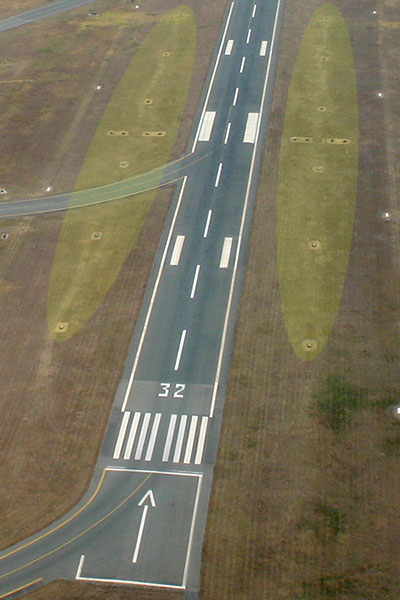
\includegraphics[width=0.4\textwidth]{06.radionavegacion/Imagenes/06.VASIS/BN-32-14-showing-T-VASIS-1-8-07.jpg} \label{fig:T-VasisAeropuerto} }
\qquad
\subfigure[T-Vasis caja de luz \protect\cite{T-VasisCajaLuz}]{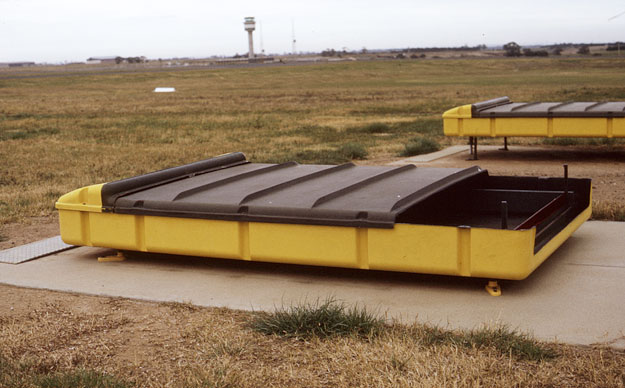
\includegraphics[width=0.4\textwidth]{06.radionavegacion/Imagenes/06.VASIS/Melbourne-T-VASIS-Type-B-bar-box-8-72-CAHS-Byron-Sullivan.jpg} \label{fig:T-VasisCajaLuz} }

\subfigure[T-Vasis Layout \protect\cite{Anexo14Vol1}]{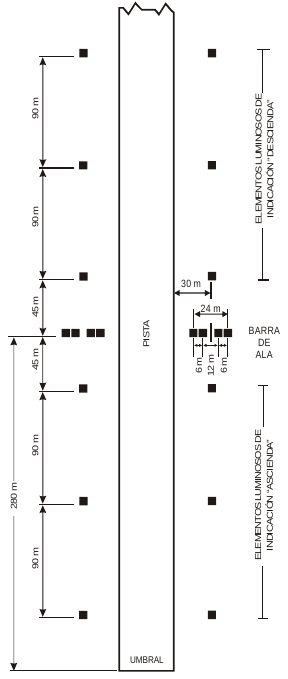
\includegraphics[angle=-90, width=0.9\textwidth]{06.radionavegacion/Imagenes/06.VASIS/06-T-Vasis-emplazamientoOACI.png} \label{fig:T-VasisLayout} }

  \caption{T-Vasis}
  \label{fig:t-vasis}
\end{figure}



% \begin{tcolorbox}[title={OACI, Anexo 14. Volumen I. Edición 2018.} ]

%   \begin{description}
%   \item[5.3.5.2] Los sistemas visuales indicadores de pendiente de aproximación normalizados consistirán en lo siguiente:
%     \begin{enumerate}[a)]
%     \item  T-VASIS y AT-VASIS que se ajusten a las especificaciones
%       contenidas en 5.3.5.7 a 5.3.5.23 inclusive; 
%     \item  PAPI y APAPI que  se ajusten a las especificaciones contenidas en 5.3.5.24 a
%       5.3.5.41 inclusive; según se indica en la Figura xxxx.
% \end{enumerate}
% \item[5.3.5.3] Se instalarán PAPI, T-VASIS o AT-VASIS si el número de clave es 3 ó 4 o cuando existe una o más de las
% condiciones especificadas en 5.3.5.1. 
%   \end{description}

% \end{tcolorbox}  

% \begin{tcolorbox}[colback=red!5!white, colframe=red!75!black,fonttitle=\bfseries,
%   title={OACI, Anexo 14. Volumen I. Edición 2018.}]
%   \begin{description}
%   \item [5.3.5.4 Recomendación.] A partir del 1 de enero de 2020,
%     debería discontinuarse el uso de T-VASIS y AT-VASIS como sistemas
%     indicadores de pendiente en aproximación visual.
% \end{description}

% \end{tcolorbox}


\subsubsection{Indicador de Trayectoria de Aproximación de Precisión}
\label{sec:06.02.03.PAPI}

También conocido como PAPI (Precision Approach Path Indicator), es un sistema más moderno de indicación
de pendiente de aproximación.

Fué desarrollado en 1974 por Tony Smith y David Johnson de la Royal Aircraft Establishment en Bedford, Inglaterra,
siendo necesarios más de dos años para su completa operatividad, que se remonta a mediados del año 1977
cuando se puso a prueba en el aeropuerto de Gatwick en Londres el prototipo de un sistema visual de aproximación
que proporcionaba datos de la senda de planeo (el primer PAPI).

%Fabricado por ADB, se observó que sus señales eran más precisas que las del sistema VASIS existente hasta el momento, que era operativo hasta unos 200 pies frente a los  50 pies del PAPI.

Consiste en cuatro conjuntos de luces alineados en forma perpendicular a la pista de aterrizaje.
Funciona básicamente del mismo modo en que lo hace el VASIS estándar, pero las luces adicionales
indican al piloto que tan alejado de la trayectoria de aproximación ideal se encuentra la aeronave.
En la Figura \ref{fig:PAPI.layout} se observa el layout según OACI.

Cuando los dos conjuntos de luces más alejados se ven rojos y los más cercanos blancos,
la aeronave está exactamente en la trayectoria de aproximación.
Cuando los tres conjuntos de luces más
alejados se ven rojos, se encuentra apenas por debajo, mientras que si los tres conjuntos de luces
más próximos se ven blancos, la aeronave está apenas por encima de la trayectoria de aproximación.
Cuatro conjuntos de luces rojas indican que está muy por debajo de la trayectoria de aproximación,
y cuatro conjuntos de luces blancas indican que está muy por encima. La mayoría de los aeropuertos
importantes utilizan este sistema.

El PAPI es colocado generalmente del lado izquierdo de la pista de aterrizaje/despegue y puede
ser visto desde una distancia máxima de 5 nm durante el día y a una distancia máxima de
20 nm de noche. Tiene dos o cuatro cajas de luces colocadas en una única fila, lo que lo
diferencia del VASIS que tiene dos filas: una más próxima y otra más alejada.

Cada caja de luces está equipada con un mecanismo óptico que divide la luz emitida en dos
segmentos, rojo y blanco. Dependiendo del ángulo de aproximación, las luces se verán o rojas o
blancas desde la posición del piloto. Lo ideal sería que las luces visibles se muevan entre el rango de
todas blancas y de la mitad rojas, cambiando a rojo sucesivamente de derecha a izquierda. El piloto
alcanza la normal trayectoria de aproximación (generalmente de 3º) cuando la mitad de las
luces sean rojas y la otra mitad blancas. Si está por debajo de la trayectoria de aproximación, las
luces rojas sobrepasarán en cantidad a las blancas, si está por encima, observará más luces blancas.

El PAPI se basa en el principio de la Lente de Fresnel.

\begin{tcolorbox}[title = {Lente de Fresnel}
  ]
  % \begin{minipage}[c]{0.6\linewidth}
  { \footnotesize
Las lentes convergentes pueden producir imágenes ampliadas cuando la distancia del objeto a la lente es menor que la distancia focal de la lente. Cuanto más corta sea la distancia focal de una lente convergente, mayor será el aumento que se puede obtener con ella. Por tanto, para obtener un aumento muy grande, se requiere una lente con un radio de curvatura pequeño y esto implica una lente muy gruesa.

La lente Fresnel tiene un perfil que le permite tener una distancia focal corta, pero con un grosor mucho menor que una lente esférica equivalente. El perfil de una lente de Fresnel se muestra en la figura. Efectivamente, es como si este perfil se formara dividiendo la superficie continua de una lente convexa convencional en varios anillos concéntricos, cada uno con la misma curvatura que la lente, pero con discontinuidades entre ellos. Dado que las refracciones que se producen en una lente dependen de su curvatura, la lente de Fresnel tendrá la misma distancia focal que la lente convexa equivalente.
}
%\end{minipage}
%\begin{minipage}[c]{0.3\linewidth}
  \begin{center}
%
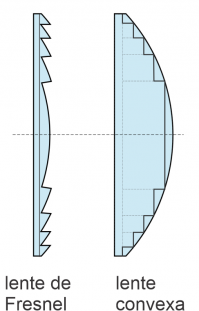
\includegraphics[height = 8cm ]{06.radionavegacion/Imagenes/06.03.ils.imagenes/FresnelLente.png}
\includegraphics[height = 8cm ]{06.radionavegacion/Imagenes/06.03.ils.imagenes/Intensidad_del_lente_de_fresnel.gif}
 \end{center}
%

%\end{minipage}
\end{tcolorbox}



El estándar para el PAPI de la FAA es el mismo que corresponde al VASIS OACI.

\href{https://adbsafegate.com/documents/2116/en/manual-voltage-powered-papi}{Manual ADB Safegate de PAPI}


\begin{figure}[!htb]
  \centering
    \includegraphics[width=0.9\textwidth]{06.radionavegacion/Imagenes/06.PAPI/PapiLayoutOACI.pdf}
    \label{fig:PAPI.layout}
  \caption{PAPI layout \protect\cite{Anexo14Vol1} }
\end{figure}



\subsection{Ayudas radioeléctricas}
\label{sec:06.03.ayudas.radioelectricas}

Entre las ayudas radioeléctricas, la que se ha utilizado por los últimos sesenta años y se encuentra
normalizada por la OACI, es el ILS. En algunos aeropuertos, sobre todo militares, es complementado
con un sistema radárico denominado PAR.
%El ILS esta siendo sustituido por el MLS que proporciona prestaciones superiores.


\begin{figure}[!h]
  \centering
  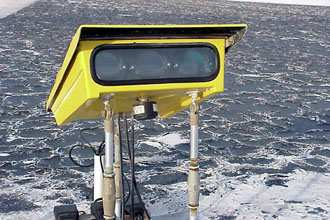
\includegraphics[height= 5cm]{06.radionavegacion/Imagenes/06.PAPI/PAPI001.png}
  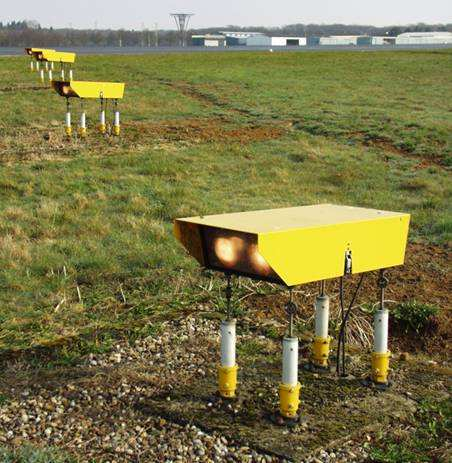
\includegraphics[height= 5cm]{06.radionavegacion/Imagenes/06.PAPI/PAPI002.png}
  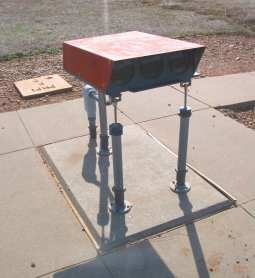
\includegraphics[height= 5cm]{06.radionavegacion/Imagenes/06.PAPI/PAPI003.png}

  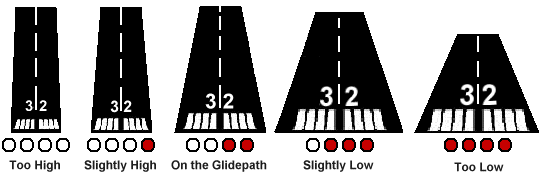
\includegraphics[height= 5cm]{06.radionavegacion/Imagenes/06.PAPI/PAPI004.png}    
  \caption{Sistema PAPI.}
  \label{fig:06.Sistemas.Aproximacion.PAPI}
\end{figure}

\subsection{Precision Approach Radar - PAR}
\label{sec:06.sistema.PAR}

El sistema de aproximación PAR, conocido en algunos aeropuertos como GCA (Ground Control
Approach), tiene una aplicación muy reducida en la actualidad, usualmente militares.
Consiste en un radar primario que proporciona la localización relativa de la aeronave respecto al sistema
emisor. La posición del avión la proporciona en telemetría, ángulo acimutal y cenital. En aplicaciones
militares se utilizan equipos como AN/FPN-63, AN/MPN, o AN/TPN-22. El alcance del sistema es
de 10 a 20 Nm (18,52 - 37,04 km).

El PAR utiliza los principios de funcionamiento del  Radar Primario de Vigilancia (Primary Surveillance Radar, PSR), la antena emite pulsos que son reflejados por la aeronave y, al recibir estos ecos, se determinan la distancia y el acimut. Sin embargo, el PAR tiene algunas características específicas:

\begin{itemize}
\item Es mucho más preciso que los PSR de vigilancia. Esto es   necesario debido a su propósito y se logra mediante la frecuencia   portadora más alta (del orden de 10 GHz en comparación con, por   ejemplo, 3 GHz para un terminal PSR) que permite un haz más   estrecho.  
\item Determina la posición de la aeronave en 3D (es decir, la   distancia desde la toma de contacto, la posición a la   izquierda/derecha de la prolongación del eje de la pista y por   encima/por debajo de la trayectoria de planeo). En sistemas más   antiguos, esto se logra agregando una segunda antena (vertical) que   proporciona la distancia y el ángulo de elevación. Se utilizan para calcular la altura geométrica de la   aeronave. También hay disponibles opciones más sofisticadas. Estos   utilizan conjuntos de antenas con dirección electrónica del haz, lo   que significa que hay menos (o ninguna) pieza móvil.  
\item Tiene una tasa   de actualización más alta. Mientras que una antena de radar terminal   normalmente gira a 10-12 rpm, el PAR solo barre un sector de unos 20º (entre 10º a la izquierda de la línea central y 10º a la   derecha) y, por lo tanto, actualiza la posición del objetivo con más   frecuencia.

  \end{itemize}



En la Figura \ref{fig:PAR.ejemplo} se puede observar una antena horizontal y otra vertical. La horizontal barre a izquierda y derecha y proporciona distancia y acimut. La antena vertical barre hacia arriba y hacia abajo y determina la altura usando el ángulo de elevación de la antena y la distancia del objetivo.

El piloto no recibe indicación alguna en la cabina, la información para la corrección de la trayectoria la recibe por radio desde la estación terrestre, que es la única que dispone de información visual en sus pantallas.

El controlador compara la posición y la altura de la aeronave con las requeridas y proporciona retroalimentación a la tripulación de vuelo en intervalos de tiempo cortos.

El dispositivo de presentación de la información para el operador se denomina \emph{escaneador Beta Scope},  la información obtenida del PAR se muestra en dos separadas en un tubo de imagen, basadas en coordenadas rectangulares. La imagen superior es una vista lateral con la línea imaginaria de la aproximación al punto de toma de contacto en la pista como línea de referencia. Esta imagen superior muestra los datos obtenidos por la antena para la detección de la altitud. Por lo tanto, también se denomina imagen de elevación.

Por su parte, la imagen inferior es la vista superior de la extensión imaginaria de la línea central de la pista, el punto de toma de contacto y los marcadores de distancia. Esta imagen inferior muestra los datos recogidos por la antena para la exploración horizontal de sectores. Por lo tanto, también se denomina imagen acimutal.

La forma histórica con tubo de imagen se sustituye ahora por una visualización asistida por ordenador en un monitor de ordenador que, sin embargo, sigue las especificaciones geométricas de la visualización con tubo de imagen.

En la Figura \ref{fig:PAR.presentacion} se presenta un ejemplo genérico de una presentación para el operador.


Durante muchos años la maniobra de aproximación a un aeródromo ha sido realizada utilizando varios sistemas: por un lado observando las indicaciones de cabina del sistema ILS y por otro, escuchando las órdenes de corrección detalladas por el personal de servicio en el GCA o PAR. Según la OACI, el PAR no es un sistema certificado, sino que puede servir como sistema de ayuda complementario al ILS, el cual es el sistema reconocido internacionalmente.

\begin{figure}[!h]\centering
  
\subfigure[ Reflejo de un operador de tráfico PAR]{ 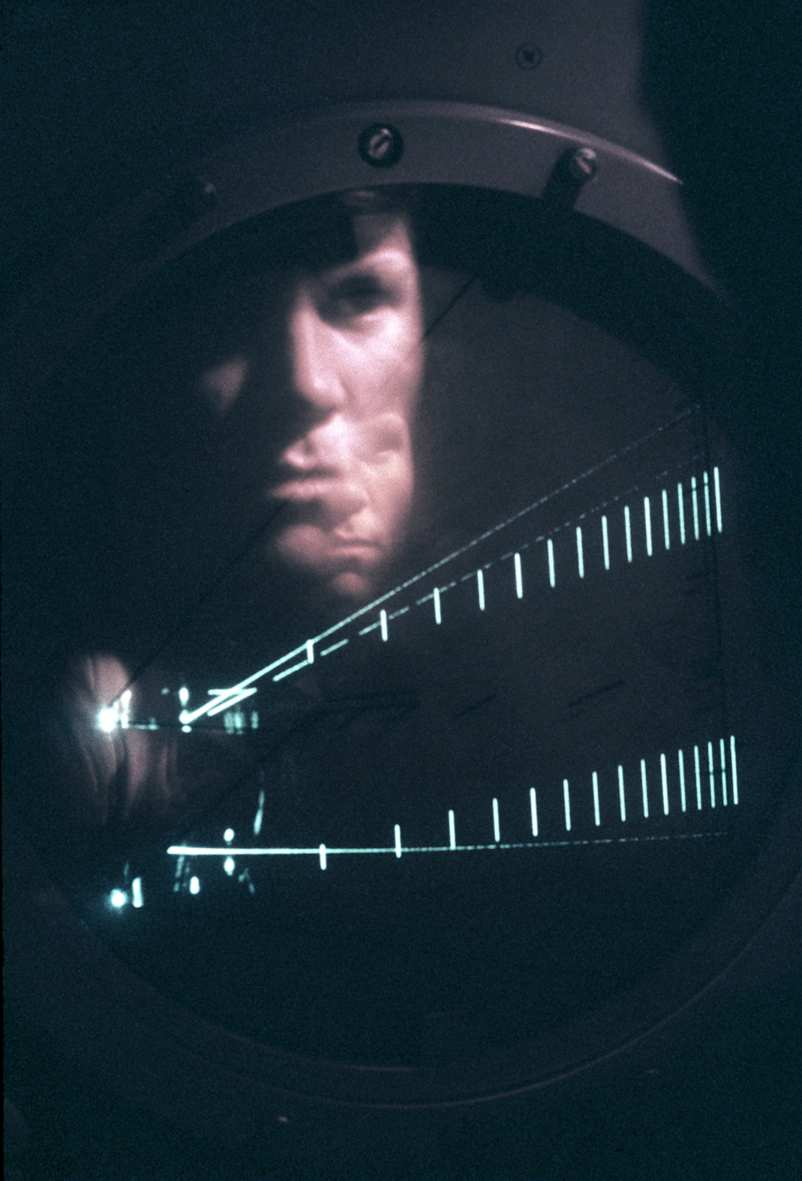
\includegraphics[height= 5cm]{06.radionavegacion/Imagenes/06.Sistemas.Aproximacion/PAR001.png}    }
\subfigure[ Ejemplo de antenas sistema PAR]{ 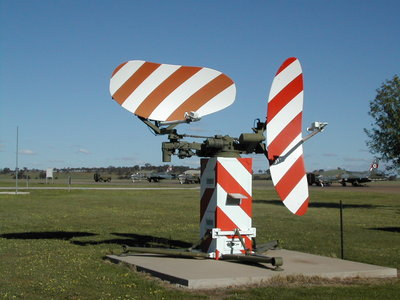
\includegraphics[height= 5cm]{06.radionavegacion/Imagenes/06.Sistemas.Aproximacion/PAR002.jpg} \label{fig:PAR.ejemplo}
  }
\subfigure[ Presentación en pantalla de un PAR]{ 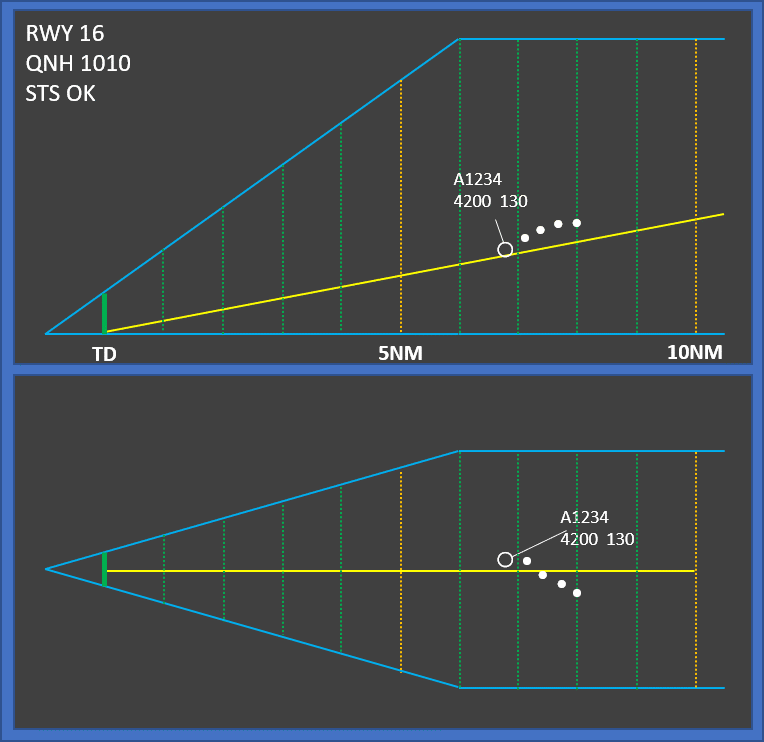
\includegraphics[height= 5cm]{06.radionavegacion/Imagenes/06.Sistemas.Aproximacion/PAR003.png} \label{fig:PAR.presentacion}
  }
  \caption{Sistema PAR}
  \label{fig:06.PAR}
\end{figure}

% hipervínculos con + información sobre PAR
% https://www.radartutorial.eu/02.basics/rp30.es.html
% https://www.radartutorial.eu/12.scopes/sc14.es.html

\subsection{Sistema de Aterrizaje Instrumental - ILS}
\label{sec:06.ILS}

\subsubsection{Un poco de historia...}
\label{sec:06.ILS.historia}

El sistema de aterrizaje instrumental (o ILS, del inglés: Instrument Landing System) es un sistema de control que permite que un avión sea guiado con precisión durante la aproximación a la pista de aterrizaje y, en algunos casos, a lo largo de la misma.

Transcurridos pocos años desde el primer vuelo realizado por los hermanos Wright en diciembre de 1903, y con los primeros pasos de la aviación comercial, empezó a sentirse la necesidad de disponer de sistemas que permitiesen volar en condiciones meteorológicas adversas y de esta forma aprovechar la ventaja de velocidad que tenían los aviones.

La aproximación para el aterrizaje fué reconocida como una de las maniobras más críticas por la cantidad de accidentes que se producían en la misma. En una película de 1939 denominada \href{https://www.youtube.com/watch?v=g7MbduUCKDA}{ \emph{Sólo los ángeles tienen alas}} se relata este problema.

%https://www.youtube.com/watch?v=g7MbduUCKDA


El rápido desarrollo que durante los primeros años del siglo XX tuvieron los sistemas de radiodifusión, permitió la puesta en marcha de los primeros sistemas de radionavegación.

En el año 1907 se concede en Alemania una patente a Otto Scheller, director técnico de la compañía C. Lorenz (más tarde Standard Elektrik Lorenz), para un sistema de radionavegación direccional. Este sistema estaba formado por dos transmisores direccionales transmitiendo en la misma frecuencia y con la misma potencia, pero con las antenas colocadas formando un cierto ángulo una respecto a la otra y emitiendo señales  de forma alternativa. Eligiendo adecuadamente el ángulo entre las antenas, se produce una línea de igual intensidad de señal (equiseñal) en el corte de los dos diagramas de radiación. Si las señales emitidas eran rayas cortas para un transmisor y rayas largas para el otro, un receptor situado en la línea de igual señal recibiría un tono continuo. Al desplazarse de esa línea predominaría la señal de uno de los transmisores dependiendo de a que lado se encontrase el receptor, ver Figura \ref{fig:seniales.lorenz}.

En el año 1919 en Estados Unidos, F. H. Engel y F. Dunmore utilizaron el principio de ``\emph{zona de equiseñal} `` para realizar una prueba de vuelo alineado con la pista. Los transmisores radiaban en la frecuencia de 300 Khz. y las señales de manipulación consistían en las letras ``\emph{A}'' (.-) y ``\emph{N}'' (-.) en código Morse, ver Figura \ref{fig:06.ILS.zonas.equisenial}.

\begin{figure}[!h]
  \centering
  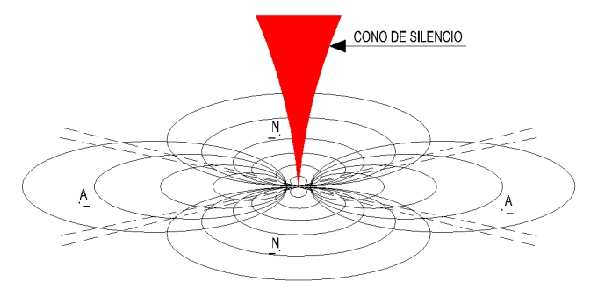
\includegraphics[width = 0.6\textwidth]{06.radionavegacion/Imagenes/06.Sistemas.Aproximacion/06_ils_zonasEquisenial.png}
    \caption{Zonas de equiseñal}
  \label{fig:06.ILS.zonas.equisenial}
\end{figure}

Durante la década de 1920 se publicaron en  Europa y América diversos artículos  describiendo sistemas experimentales de ``\emph{aterrizaje automático}''.


Bajo la responsabilidad de la Oficina de Normas del Departamento de Comercio de Estados
Unidos y con el apoyo de la Fundación Guggenhein, durante el año 1929, se instaló en Mitchel Field
un localizador consistente en un sistema equiseñal alineado con el eje de la pista, en el que se habían
añadido a las letras en código Morse dos señales de modulación de frecuencias establecidas en 65 Hz
y 86,7 Hz, y una radiobaliza de baja potencia para señalar el punto a partir del cual podía iniciarse
el descenso seguro a la pista.

Para las pruebas en vuelo se utilizó un avión biplano de entrenamiento Consolidated PT-3 equipado con tres instrumentos especiales: un horizonte artificial, un giróscopo y un altimetro barométrico graduado en intervalos de 3 m. Ademas se instaló el receptor del localizador cuyas emisiones se mostraban por medio de dos láminas vibrantes mecánicamente ajustadas a las frecuencias de modulación de la estación de tierra y manipuladas por pequeños electroimanes conectados al circuito de salida del receptor.

Cuando se recibían las señales del localizador, las láminas vibraban con una amplitud proporcional a la intensidad de las señales recibidas. Cuando se volaba en la prolongación del eje de pista
(curso) las vibraciones de las dos láminas tenían igual amplitud. Al desplazarse del curso, vibraba
con mayor amplitud la lámina ajustada a la frecuencia que predominaba en ese lado.

\begin{tcolorbox}
El 24 de septiembre de 1929, el Teniente James Doolittle realizó en el Consolidated PT-3 una serie de aterrizajes, sentado en el asiento trasero del mismo, con la cabina completamente cubierta y guiándose exclusivamente
con los instrumentos de abordo. Había comenzado el aterrizaje instrumental. \vspace{3mm}

\begin{minipage}[c]{0.3\linewidth}
    
\includegraphics[width = 0.9\linewidth]{06.radionavegacion/Imagenes/06.Sistemas.Aproximacion/06_Doolittle.png}
\captionof{figure}{James Doolittle}
\end{minipage}
\begin{minipage}[c]{0.7\linewidth}
  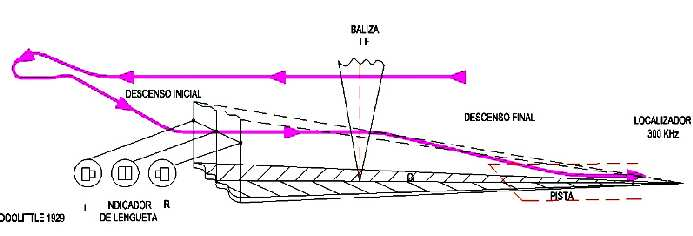
\includegraphics[width = \linewidth]{06.radionavegacion/Imagenes/06.Sistemas.Aproximacion/06_Doolittle_vuelo_1929.png}
  \captionof{figure}{Vuelo de Doolittle en 1929}
\end{minipage}

\end{tcolorbox}

Estos trabajos iniciales dieron un nuevo impulso a la investigación en Europa. Así en el año 1932
el Dr. Ernst Kramer de Lorenz patentó un sistema combinado de localizador (información de azimut)
y senda de planeo (información de elevación) verticalmente polarizado que operaba en la frecuencia
de 33,3 Mhz. En el localizador, instalado en el extremo de la pista y de tipo equiseñal, la portadora
estaba modulada por una señal de 1150 Hz que se manipulaba con las letras ``\emph{E}'' ( . ) y ``\emph{T}'' ( - ) en código Morse. Además de la información acústica, en el panel de instrumentos del avión se introdujo
una indicación visual de la posición respecto al eje de pista por medio de una aguja.
La senda de planeo era del tipo ``\emph{intensidad constante}'' y originalmente consistía en el borde
inferior del lóbulo formado por la superposición de los diagramas del localizador. El piloto tenía que
seguir la trayectoria determinada por los puntos del espacio en los que detectaba una intensidad
constante indicada en un instrumento.

Durante el invierno del año 1932-33 Lufthansa realizó varios vuelos de prueba utilizando este
sistema instalado en el aeropuerto de Berlin - Tempelhof.
Con el fin de mejorar la información de la trayectoria de planeo, en 1937 la compañía Lorenz dio
forma a una patente del Dr. Kramar consistente en un transmisor en UHF conectado a dos antenas
colocadas una encima de la otra y que radiaban alternativamente. De esta forma se generaban en el
espacio dos lóbulos cuya intersección formaba un haz en la trayectoria de descenso de 3º .

Esta era
la senda de planeo equiseñal que se reinventó en Estados Unidos en 1940.
En Estados Unidos se probaron distintas versiones entre los años 1931 a 1937.
En la Figura \ref{fig:06.ILS.Lorenz.1938}
 puede verse el esquema de un sistema que estaba formado por un transmisor como localizador
en la frecuencia de 300 KHz y otro como senda de planeo de intensidad constante a 93,7 Mhz. A
este sistema instalado en varios aeropuertos de Estados Unidos y Europa se le encontraron grandes
limitaciones debido principalmente a problemas por reflexiones de las señales.

\begin{figure}[!h]
  \centering
  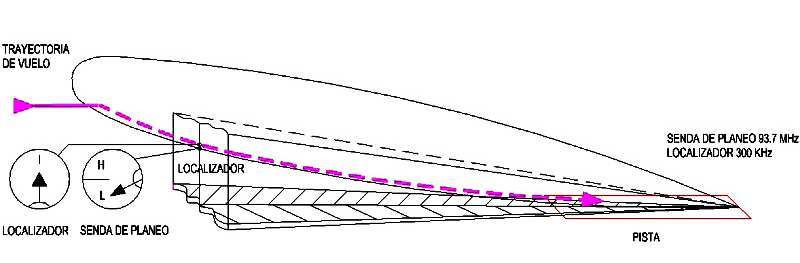
\includegraphics[width = 0.9\textwidth]{06.radionavegacion/Imagenes/06.Sistemas.Aproximacion/06_1938.png}
    \caption{Lorenz, año 1938}
  \label{fig:06.ILS.Lorenz.1938}
\end{figure}

En el año 1938 se desarrollo otro sistema de aterrizaje sin visibilidad por Irving Metcalf de la
Oficina de Comercio Aéreo de Estados Unidos con el apoyo del Massachusetts Institute of Technology.
Este tipo de sistema de aterrizaje por instrumentos basaba en un transmisor situado en el aeropuerto
que producía un blanco en una pantalla de rayos catódicos situada en la aeronave. También se
presentaban en la pantalla otros blancos que se obtenían de un giróscopo direccional y de un horizonte
artificial.

Así, al aproximarse el avión a tierra, la pantalla presentaba el cambio aparente de posición
del transmisor con respecto al horizonte. Tras las primeras pruebas, este sistema fue abandonado.
También en 1938, Lorenz junto con la International Telephon and Telegraph (ITT) inició un
proyecto, financiado por la Civil Aviation Administration (CAA) de Estados Unidos, para desarrollar
un sistema formado por un localizador horizontalmente polarizado radiando en la frecuencia de 110
Mhz, una senda de planeo de intensidad constante a 93,9 Mhz que proporcionaba una trayectoria de
decenso de tipo parábola y una radiobaliza de 75 Mhz. En este sistema ya se habian adoptado las
frecuencias de 90 Hz y 150 Hz para los tonos que, por medio de un modulador mecánico consistente
en dos ruedas con 3 y 5 álabes respectivamente y que giraban movidas por un motor sincrono,
modulaban a la portadora.

En 1939 el sistema se completó con supervisión y control remoto y se
instaló en el aeropuerto de Indianapolis, llevandose a cabo un programa de pruebas con un Boeing 247D equipado con receptores y registradores para evaluar las señales. El localizador y las radiobalizas
eran en principio iguales a las utilizadas hoy en día.
Alentados por los resultados obtenidos con la senda de planeo de intensidad constante, la CAA
llegó a un acuerdo con ITT para desarrollar un sistema de senda de planeo equiseñal en la frecuencia
de 330 Mhz consiguiendolo en 1941.

En esta Senda de Planeo equiseñal, la portadora de 330 Mhz se separaba en dos canales cada uno
de los cuales se modulaba con un tono de 90 Hz o de 150 Hz. El sistema radiante estaba formado por
dos antenas montadas en un mástil vertical. La antena inferior se colocaba a una altura de 1,8 m del
suelo y se alimentaba con la señal modulada con 90 Hz, la antena superior estaba a aproximadamente
8 m del suelo y se alimentaba con la señal modulada con 150 Hz.

\begin{figure}[!h]
  \centering
  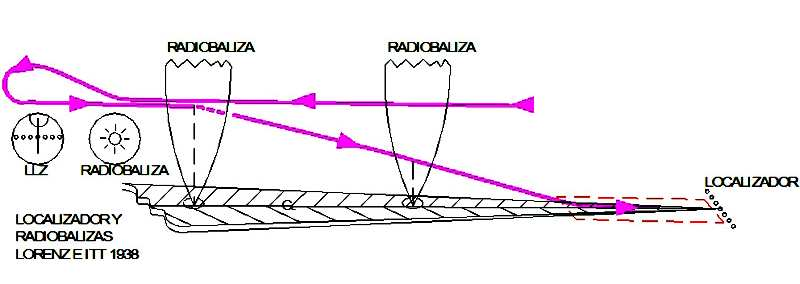
\includegraphics[width = 0.9\textwidth]{06.radionavegacion/Imagenes/06.Sistemas.Aproximacion/06_1941.png}
    \caption{ Año 1941}
  \label{fig:06.ILS.1941}
\end{figure}

Utilizando la reflexión en el terreno se producian dos diagramas de radiación de tal forma que,
modificando las alturas y las amplitudes de las señales que alimentaban a las antenas, se variaban
estos diagramas para obtener una linea de puntos de equiseñal en el ángulo de la trayectoria de
descenso. Por debajo de la trayectoria predominaba la señal de 150 Hz y por encima la de 90 Hz.
Durante los años de la II Guerra Mundial, se realizaron diversos desarrollos de sistemas militares
portatiles basados en el sistema civil de ITT.

También hubo otros desarrollos como el realizado por Sperry en Estados Unidos y consistente en
un localizador y senda de planeo equiseñal en la frecuencia de 3000 Mhz.

Finalmente en el año 1943 se tomó una decisión para estandarizar un sistema de aterrizaje por
instrumentos (ILS: Instrument Landing System) y la opción seleccionada fue la presentada por ITT
trabajando en VHF y UHF y denominada SCS-51.

El SCS-51, como el sistema de Lorenz, estaba basado en una radiación en VHF formada por dos
diagramas de onda continua (CW: continous wave) que se superponian y formaban un haz en acimut
conocido como Localizador (LLZ). Había otra segunda radiación en UHF formada por otros dos
diagramas que formaban un haz en el plano vertical llamado Senda de Planeo (GP). Por tanto el ILS
no solo proporcionaba información de guiado acimutal, sino que también daba información de guiado
en la trayectoria de descenso. La diferencia básica entre el ILS y el sistema de Lorenz era que sus dos
diagramas estaban polarizados horizontalmente y modulados por tonos en vez de manipulados con
señales Morse. El ILS tenía la ventaja de dar una indicación del grado de divergencia respecto al eje
en vez de solo indicar si el avión se encontraba a un lado o a otro del eje como hacían los primeros
sistemas.

En 1944 mientras en Gran Bretaña se realizaban pruebas con un prototipo de SCS-51, se modificaba un sistema de radar Rebecca-Eureka para convertirlo en un Equipo Medidor de Distancias
(DME :Distance Measuring Equipment).

Al final de la Segunda Guerra Mundial se realizaron esfuerzos para adaptar las experiencias y equipos
desarrollados en el campo militar a un uso civil. Fruto de estos trabajos el ILS se convirtió en el
sistema normalizado de aterrizaje por instrumentos cuando se celebró la reunión de la OACI en Chicago en el año 1946, incluyéndolo en su Anexo 10 al Convenio sobre Aviación Civil Internacional titulado ``\emph{Telecomunicaciones Aeronáuticas}''. En 1949
fue aceptado por la OACI como sistema de aproximación.


\begin{figure}[!h]
  \centering
  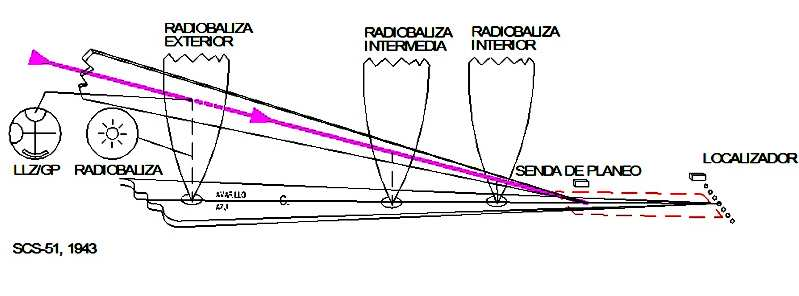
\includegraphics[width = 0.9\textwidth]{06.radionavegacion/Imagenes/06.Sistemas.Aproximacion/06_1943.png}
    \caption{ Año 1943}
  \label{fig:06.ILS.1943}
\end{figure}

Desde entonces los principios básicos de funcionamiento del ILS no se han modificado, si bien se
han realizado grandes avances tanto en la electrónica de los equipos que generan las señales como en
los sistemas de antenas utilizados para generar los diagramas de radiación.

Y así este sistema cuyos antecedentes empezaron a establecerse hace más de 70 años, sigue
operativo en los aeropuertos de todo el mundo posibilitando que las más modernas aeronaves realicen
aproximaciones y aterrizajes seguros y fiables en cualquier condición meteorológica.

\subsubsection{Componentes sistema ILS}
\label{sec:06.ILS.componentes}

El sistema ILS se divide en tres partes bien diferenciadas:
\begin{itemize}
\item Información de guía: se proporciona por medio del Localizador
  (LLZ), que proporciona guía lateral, y la Senda de Planeo (GS), para
  la guía vertical.
\item Información de distancia: la brindan las Balizas o el DME (Distance Measurement Equipment).
\item Información visual: la compone el sistema ALS (ver \ref{sec:06.02.01.ALS}).
\end{itemize}

Varios de estos componentes pueden verse en la Figura \ref{fig:06.ILS.sistema}.


\begin{figure}[!h]
  \centering
  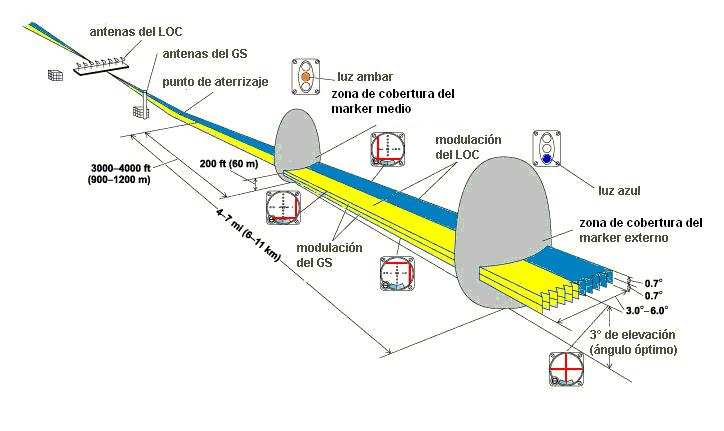
\includegraphics[width = 0.9\textwidth]{06.radionavegacion/Imagenes/06.Sistemas.Aproximacion/06_ILS.png}
    \caption{ Sistema ILS}
  \label{fig:06.ILS.sistema}
\end{figure}

Información de guía

Para la información de guía, el ILS posee dos subsistemas independientes: uno sirve para proporcionar guía lateral (Localizador) y el otro para proporcionar guía vertical.

\begin{description}
\item [\bf Localizador LLZ:] una serie de antenas localizadoras (LLZ, LOC o
  localizer) están situadas normalmente a unos 1000 pies (305 m) del
  final de la pista y suelen consistir en 8 ó 14 antenas
  direccionales, ver Figura 15. Se transmiten señales portadoras entre
  los 108 MHz y 112MHz definidas para cada localizador. Estas
  portadoras se modulan con 90 Hz y 150 Hz y con distintas fases.
  En la Figura \ref{fig:06.ILS.antenas.localizador}
  pueden observarse algunas antenas utilizadas en las aeronaves para recibir
  la señal del LLZ.
  
Esto produce el efecto que la señal de 150 Hz predomine en el lado derecho de pista y la de 90
Hz en el izquierdo, desde el punto de vista del piloto, ver Figura \ref{fig:06.ILS.sistema.patrones.emision}.
El receptor del localizador
en el avión mide la diferencia entre la modulación entre las señales de 90 Hz y 150 Hz: cuando
la diferencia es de cero, la antena receptora está en la línea central del localizador, lo que
normalmente coincide con el centro de la pista.

\begin{figure}[!htb]
  \centering
  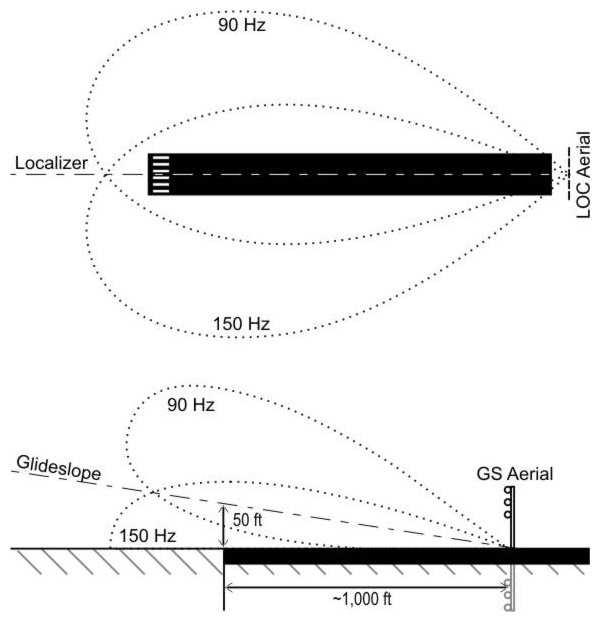
\includegraphics[width = 0.5\textwidth]{06.radionavegacion/Imagenes/06.Sistemas.Aproximacion/06_ILS_patronesEmision.png}
    \caption{ Sistema ILS. Patrones de emisión}
  \label{fig:06.ILS.sistema.patrones.emision}
\end{figure}


\begin{figure}[!htb]
  \centering
  \subfigure[Disposición del localizador y luces de aproximación en la base de la USAF Whiteman, Johnson County, Missouri]{ 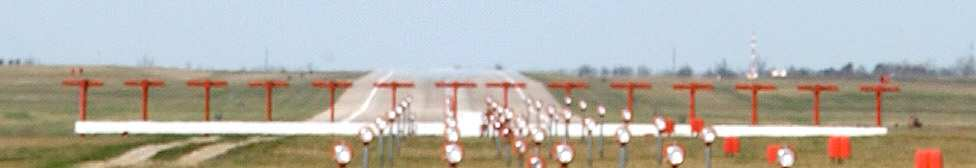
\includegraphics[width = 0.9\textwidth]{06.radionavegacion/Imagenes/06.Sistemas.Aproximacion/06_ILS_antenas_LLZ.png}  }

  \subfigure[Disposición del localizador]{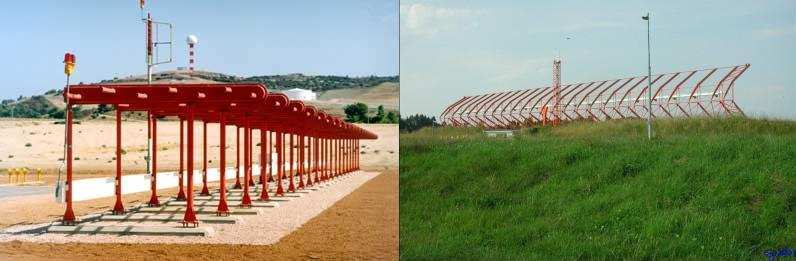
\includegraphics[width = 0.9\textwidth]{06.radionavegacion/Imagenes/06.Sistemas.Aproximacion/06_ILS_antenas_LLZ_002.png} }

  \subfigure[Algunas antenas de recepción de LLZ en el avión (también recibe la senal del VOR, que es un sistema de radionavegación)]{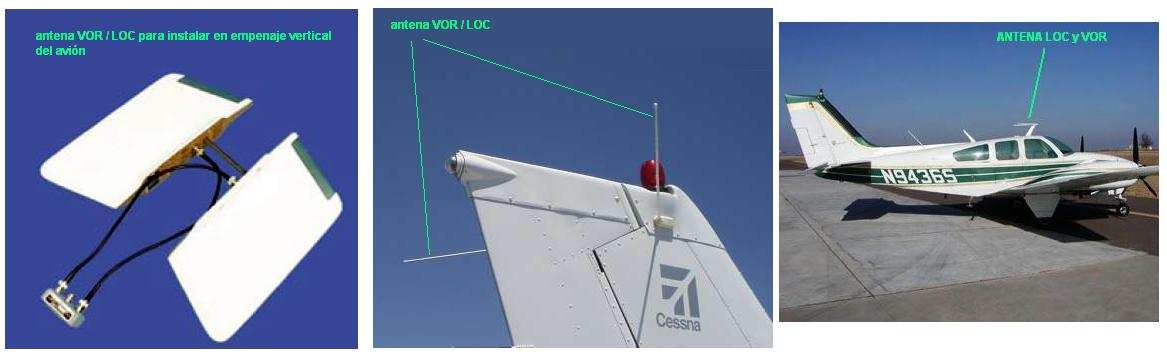
\includegraphics[width = 0.9\textwidth]{06.radionavegacion/Imagenes/06.Sistemas.Aproximacion/06_ILS_antenas_recepcion.png} }
  
  \caption{Antenas del localizador}
  \label{fig:06.ILS.antenas.localizador}
\end{figure}

\item [\bf Senda de Planeo - GS] una antena transmisora de la senda de planeo (GS, del inglés:
glideslope) se sitúa a un lado de la zona de la pista donde se produce la toma, Figura 16.
La señal GS se transmite a una frecuencia de entre 328,6 MHz y 335,4 MHz, usando una
técnica similar a la del localizador; la señal está situada para marcar una senda de planeo de
aproximadamente 3o sobre la horizontal. También se usan 2 tonos de audio de 90 y 150 Hz, en
este caso el de 90 Hz arriba y el de 150 Hz abajo. Cuando en el avión las señales de 90 y 150
Hz tienen el mismo nivel, significa que el avión desciende en el ángulo correcto,
ver Figura \ref{fig:06.ILS.sistema.patrones.emision}.

En la Figura \ref{fig:06.ILS.GS} pueden observarse algunas antenas utilizadas en las aeronaves para recibir la
señal del GS.

Las frecuencias del localizador y la senda de planeo están empareajadas de manera que sólo se
requiere seleccionar una frecuencia para sintonizar ambos receptores. El localizador proporciona
una señal de código morse transmitida a 1020 Hz para permitir la identificación. Por ejemplo,
en el aeropuerto de Barajas, se transmitiría MAA para la pista 33L. Esto permite saber si el
ILS está operando con normalidad o si está correctamente sintonizado. La señal de senda de
planeo no transmite ninguna señal de identificación, por lo que se depende del localizador.

\item [\bf Instrumental en cabina]  las señales del localizador y la senda de planeo se muestran
  en un Instrumento de la cabina llamado Indicador de Desviación de Curso (CDI, del inglés: Course
Deviation Indicator), como agujas horizontales y verticales (o un instrumento electrónico que las
simule), en la Figura 17 pueden verse algunos modelos de este instrumento. El piloto controla
el avión de manera que las agujas permanezcan centradas en el indicador, pues es entonces
cuando el avión sigue la senda de planeo y la dirección correctas. Las señales también pueden
pasarse a los sistemas de piloto automático para permitir que éste vuele la aproximación.


\begin{figure}[!htb]
  \centering
  \subfigure[Antenas de tierra del GS]{ 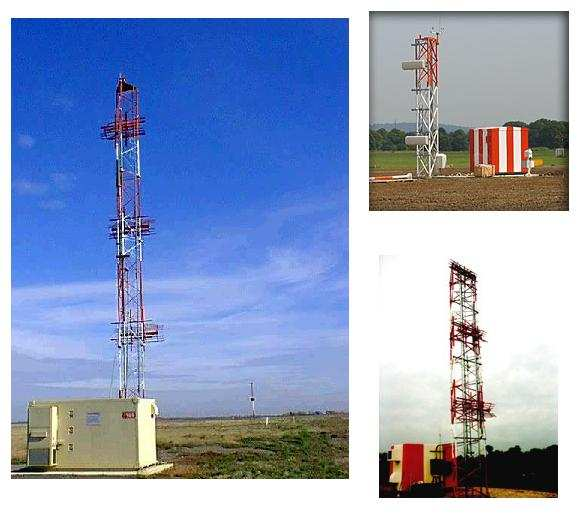
\includegraphics[width = 0.7\textwidth]{06.radionavegacion/Imagenes/06.Sistemas.Aproximacion/06_ILS_antenasTierraGS.png}  }

  \subfigure[Antenas de recepción de GS en la aeronave]{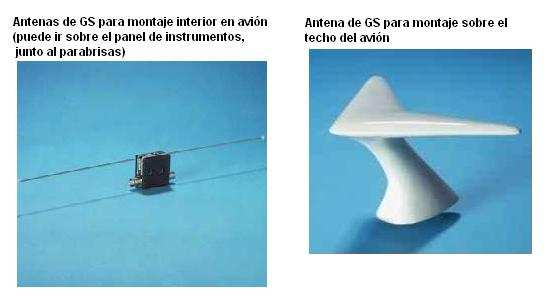
\includegraphics[width = 0.7\textwidth]{06.radionavegacion/Imagenes/06.Sistemas.Aproximacion/06_antenasAeronaveGS.png} }
  
  \caption{Antenas GS}
  \label{fig:06.ILS.GS}
\end{figure}
  
\end{description}

\subsubsection{Radiobalizas}
\label{sec:06.ILS.radiobalizas}


Las radiobalizas operan a 75 MHz y se utilizan para indicar la altura y posición aproximadas a
las que se encuentra el avión durante su aproximación.
Son tres:
\begin{description}
\item [\bf Radiobaliza exterior (OM, del inglés: outer marker)] localizada
  a 3,9 millas náuticas (7,2 km) del umbral de la pista. Emite dos
  rayas (morse) por segundo con un tono de 400 Hz; su indicador es
  azul. Se utiliza esta radiobaliza para ayudar a los chequeos de
  altura, distancia y funcionamiento del equipamiento. Se puede
  combinar con un NDB para crear una Radiobaliza Exterior de
  Localizador (LOM, del inglés: Locator Outer Marker).
  \item [\bf Radiobaliza
  intermedia (MM, del inglés: middle marker)] se localiza para que, en
  condiciones de baja visibilidad informe que el contacto con la pista
  es inminente. Está modulada con un tono de 1300 Hz y emite puntos y
  rayas (morse) alternativos. Su color es ámbar.  
\item [ \bf Radiobaliza interior  (IM, del inglés: inner marker)] cuando está instalada, se localiza
  para que en condiciones de baja visibilidad se indique que se está a
  punto de cruzar el umbral de la pista. En esta posición un avión
  normalmente llega a las condiciones mínimas de la Categoría II. La
  modulación es de puntos a 3000 Hz, 6 por segundo. Su color es
  blanco.  En la actualidad la radiobaliza interior resulta rara de
  encontrar en las instalaciones de ILS. En la Figura 13 puede
  observarse la disposición de las mismas.
\end{description}


\begin{figure}[!htb]
  \centering
  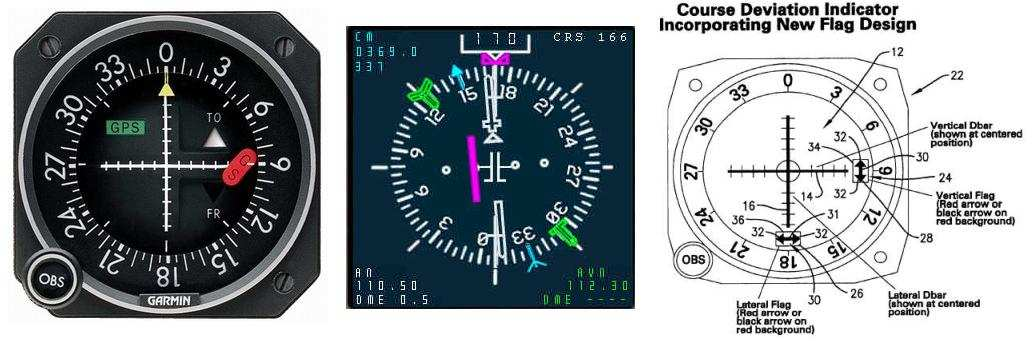
\includegraphics[width = 0.9\textwidth]{06.radionavegacion/Imagenes/06.Sistemas.Aproximacion/06_ILS_CDI.png}
  \caption{Diversos tipos de CDI}
  \label{fig:06.ILS.CDI}
\end{figure}

\subsubsection{Categorías (CAT) de ILS}
\label{sec:06.ILS.categorias}

Uno de los mayores enemigos de la navegación aérea es la baja visibilidad y especialmente en las operaciones
de aproximación, aterrizaje y despegue ya que en esos momentos es imprescindible tener referencias
visuales del entorno próximo y en particular del terreno. Cuando se conduce un automóvil con
niebla es fácil entender la sensación de un piloto realizando una aproximación a 300 o 400 km/h en
condiciones de baja visibilidad y sabiendo que el terreno cada vez está más cerca. De ahí la necesidad
de disponer de un procedimiento y unas ayudas visuales e instrumentales que le permitan terminar
el vuelo con total seguridad.

Por todo ello uno de los primeros trabajos encomendados a OACI después de su creación en
1947, fue establecer lo que se denomina como ``\emph{Operaciones Todo Tiempo}'' (AWO: All Wheather
Operations) y que la propia OACI define como: ``\emph{Todo despegue o aterrizaje realizado en condiciones
  meteorológicas que reduzcan la referencia visual}''.

\begin{tcolorbox}[title = {Categorías de aproximación de precisión de OACI}]  
En lo referente a la aproximación y el aterrizaje, las operaciones de baja visibilidad se dividen
en categorías dependiendo de los mínimos meteorológicos y de los objetivos operacionales que se
pretendan conseguir. OACI en el Adjunto C al Anexo 10 ``\emph{Telecomunicaciones aeronáuticas}'' da las
siguientes definiciones para estas categorías, ejemplos de las mismas pueden observarse en
la Figura \ref{fig:06.ILS.categoriasAproximacion}:

  \begin{description}
  \item  [\bf Categoría I (CAT I):] una altura de decisión no inferior a
    60 m (200 ft) y con visibilidad no inferior a 800 m o alcance
    visual en la pista no inferior a 550 m; 
  \item [Categoría II (CAT II):]
    una altura de decisión inferior a 60 m (200 ft), pero no inferior
    a 30 m (100 ft) y alcance visual en la pista no inferior a 300 m;
    
  \item [Categoría IIIA (CAT IIIA):] una altura de decisión inferior a 30
    m (100 ft) o sin limitación de altura de decisión y alcance visual
    en la pista no inferior a 175 m; 
  \item [Categoría IIIB (CAT IIIB):] una
    altura de decisión inferior a 15 m (50 ft) o sin limitación de
    altura de decisión y alcance visual en la pista inferior a 175 m
    pero no inferior a 50 m; y 
  \item [Categoría IIIC (CAT IIIC):] sin
    altura de decisión ni limitaciones de alcance visual en la pista.
  \end{description}
  
\end{tcolorbox}


\begin{figure}[!htb]
  \centering
  \subfigure[Condiciones metereológicas visuales]{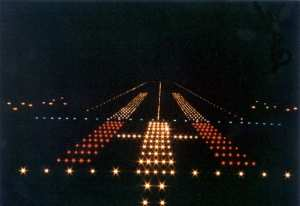
\includegraphics[height = 5cm ]{06.radionavegacion/Imagenes/06.Sistemas.Aproximacion/06_Aprox_visual_Cat0.png} }
    \subfigure[Categoría I]{
\includegraphics[height = 5cm ]{06.radionavegacion/Imagenes/06.Sistemas.Aproximacion/06_Aprox_visual_CatI.png} }

  \subfigure[Categoría II]{
\includegraphics[height = 5cm ]{06.radionavegacion/Imagenes/06.Sistemas.Aproximacion/06_Aprox_visual_CatII.png} }
  \subfigure[Categoría IIIa]{
\includegraphics[height = 5cm ]{06.radionavegacion/Imagenes/06.Sistemas.Aproximacion/06_Aprox_visual_CatIIIa.png} }

      \subfigure[Categoría IIIb]{
\includegraphics[height = 5cm ]{06.radionavegacion/Imagenes/06.Sistemas.Aproximacion/06_Aprox_visual_CatIIIb.png} }

    \caption[06.ILS.categorias.visibilidad]{Categorías de visibilidad OACI en aproximación}
  \label{fig:06.ILS.categoriasAproximacion}
\end{figure}



  % -rwxrwxrwx 1 jorge jorge  95613 ago 21 03:17 06_TableroRadiobalizas.png
  % -rwxrwxrwx 1 jorge jorge 334919 ago 21 03:17 06_ILS_antenaRadiobaliza.png

En las definiciones anteriores se entiende como altura de decisión a la del punto de la aproximación
final en el que el piloto debe decidir continuar el aterrizaje si tiene referencias visuales externas (luces
de aproximación o de pista) o iniciar una maniobra de aproximación frustrada si no las tiene. Por
otra parte el alcance visual en la pista o RVR se define como la distancia a la que un piloto situado
a 5 m de altura sobre el eje de pista, puede ver las señales de la superficie de la pista o las luces que
la delimitan o identifican su eje.

% \begin{table}[!htb]
%   \centering
%   \caption{Ventajas y desventajas del ILS}
%   \label{tab:06.ILS.ventajas+desventajas}

%   \begin{tabular}{m{0.45\textwidth}m{0.45\textwidth}} \rowcolor{cyan!40}
%   {\bf Ventajas}
%     &   {\bf Desventajas} \\ \hline
%     &
%     \begin{itemize}
%         \item  S\'olo hay 40 canales disponibles en todo el mundo.
%         \item  Los haces de azimut y senda de planeo son fijos y estrechos. Como resultado, los aviones deben estar secuenciados y separados adecuadamente, lo que provoca retrasos en el aterrizaje.
%         \item  No existen procedimientos especiales disponibles para aviones, helicópteros y aviones más lentos como los STOL.
%         \item   No puede ubicarse en áreas montañosas y requiere grandes extensiones de terreno plano y despejado para  para minimizar la interferencia con los haces del localizador y de la senda de planeo.
%         \item  Vehículos,  aeronaves en rodaje, las  que vuelan a baja altura y los edificios deben encontrarse fuera de la zona de transmisión para minimizar las desviaciones en las señales del localizador y la senda de planeo.
%    \end{itemize}
%   \end{tabular}
% \end{table}




\subsection{Sistema de Aterrizaje por Microondas (MLS)}
\label{sec:06.MLS}

\subsubsection{Un poco de historia...}
\label{sec:06.MLS.historia}

El MLS (Microwave Landing System) es un sistema similar al ILS en cuanto a su presentación en
instrumental, es decir en su utilización para los pilotos, proveyendo guía lateral y vertical a través
de los instrumentos convencionales resultando una cobertura similar a la del ILS.

Estaba predestinado a ser el ILS del futuro pero, en actualidad existen muy pocos instalados y
lo están a modo de prueba, pues su tecnología aun esta en desarrollo, de hecho la FAA ha retrasado
mucho sus planes de instalación a punto tal que su tecnología se vio superada por la del GPS.

En 1967, una comisión técnica de los Estados Unidos creó un comité para definir las especificaciones técnicas y operativas de un nuevo sistema de aproximación que superara los inconvenientes
que presentaba el ILS. El trabajo finalizó en 1972 otorgando la banda ``\emph{C}'' de microondas (5030 - 4090 Mhz) al nuevo sistema. En 1974 la OACI solicitó a sus Estados miembros reemplazar el sistema
ILS por nuevo sistema MLS, convocando un concurso internacional para proponer un sistema de
implementación. Fue en 1978 cuando un equipo australiano diseño el sistema ``\emph{TRSB}'' (Time Reference Scanning Beam), conocido en Australia como INTERSCAN (time INTERval SCANning), que
finalmente sería elegido.

\begin{figure}[!htb]
  \centering
  \subfigure[MMLS modelo AN/TRN-45]{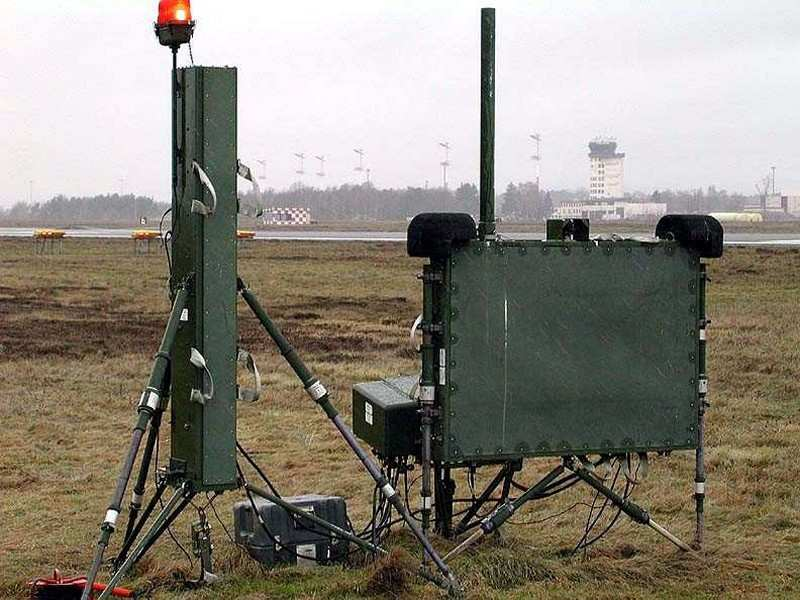
\includegraphics[height=6cm]{06.radionavegacion/Imagenes/06.Sistemas.Aproximacion/06_MLS_003.png} }
  \subfigure[ MMLS en el aeropuerto de la Universidad de Ohio (EEUU) ]{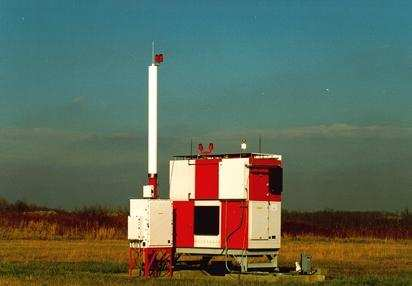
\includegraphics[height=6cm]{06.radionavegacion/Imagenes/06.Sistemas.Aproximacion/06_MLS_004.png} }

  \subfigure[MMLS estación experimental INTERSCAN (Aeropuerto Tullamarine Melbourne, Australia, 1977)]{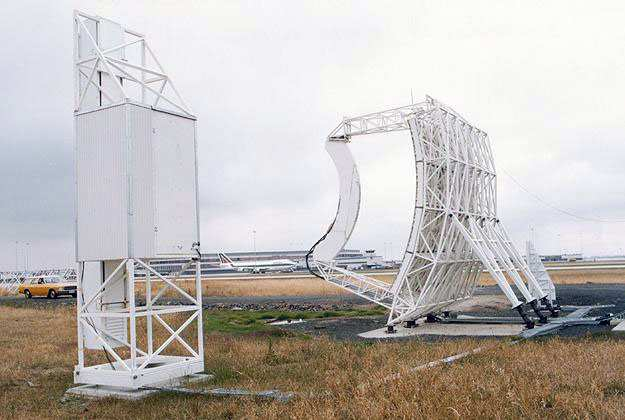
\includegraphics[height=6cm]{06.radionavegacion/Imagenes/06.Sistemas.Aproximacion/06_MLS_005.png} }

  
  \caption{Estaciones terrestres de MLS}
  \label{fig:06.MLS.estaciones}
\end{figure}



En 1985 la OACI adoptó el estandard MLS recomendando la transición de ILS a MLS para
1998, sin embargo, la etapa de pruebas a la que estaba sometido fue alargando poco a poco su
implementación definitiva. Como consecuencia de la aparición de los sistemas de navegación por
satélite, y el resultado de algunas pruebas realizadas para facilitar la maniobra de aterrizaje, el MLS
entró en una crisis que casi lo hizo desaparecer. No obstante, la falta de precisión del GPS en el
momento de la toma le ha vuelto a otorgar al MLS un hueco dentro del panorama de los sistemas
de navegación.

Así, la OACI, que estaba al corriente de los acontecimientos, decidió recomendar en 1995 que
los estandares ILS y MLS convivieran durante 15 o 20 años más, hasta que los sistemas por satélite
confirieran la seguridad y precisión necesarias. Hoy en día, aeronaves de última generación como el
Airbus A380 o el A400M han sustituido el ILS por el MLS. En otras aeronaves se integran el ILS
con el MLS.

Existen diversas variedades de MLS, se tiene un equipo móvil militar denominado MMLS (Mobile
MLS), que se despliega en tiempo record para los emplazamientos que carezcan del sistema. Igualmente se dispone de otra variedad militar del MLS que transmite en la banda Ku de 15 GHz, cuyas
antenas son de menor diámetro y, por lo tanto, más portables.
Las transmisiones se realizan en SHF (banda de microondas) en frecuencias comprendidas entre
5031 y 5091 MHz por lo que en principio no podrán ser captados por los receptores del ILS, esto
espera ser superado de alguna forma, principalmente por modificación de dichos receptores. Además
esta equipado con un nuevo DME denominado DME-P.

El sistema se basa en el barrido del sector de entrada de la pista por medio de una antena de
barrido horizontal, la onda portadora esta modulada en frecuencia variable de acuerdo al ángulo, para
que luego el receptor en el avión en base a la frecuencia de la portadora pueda calcular mediante una
relación matemática.

La diferencia mas notoria respecto del ILS es que ademas de proveer una trayectoria rectilínea
como el ILS puede también marcar una trayectoria en curva.

\subsubsection{Equipo de tierra}
\label{sec:06.MLS.equipoTierra}

El equipo de tierra se compone de varios subconjuntos:

\begin{description}
\item [\bf Equipo de acimut:] proporciona el guiado horizontal y la posición
  de la aeronave respecto al eje de la pista. El piloto puede
  seleccionar el ángulo por el que desea ingresar en la pista.

\item [\bf Equipo de elevación:] Realiza el guiado vertical durante la aproximación, pudiendo el piloto
seleccionar el ángulo de descenso.

\item [\bf Equipo de azimut posterior:] informa al piloto de la trayectoria que ha de seguir durante la
aproximación frustrada para volver a intentar un nuevo aterrizaje.

\item [\bf Equipo de transmisión de palabras de datos:] notifica al equipo de abordo toda la información necesaria para calcular la maniobra a realizar.

\item [\bf Equipo DME:] es el equipo medidor de distancia que, para este caso, se considera como
subconjunto del MSL. Entre las modificaciones que se le han hecho se encuentra la incorporación
del nuevo DME-P.

\end{description}

Todos los subconjuntos se localizan en cinco posiciones diferentes del aeropuerto. Por un lado
cuatro radiofaros y por el otro, separada del resto, la estación central que sincroniza los radiofaros
anteriores y transmite las señales de identificación, los datos básicos y auxiliares, las señales de
indicación de ``\emph{fuera de cobertura}''.

Los cuatro radiofaros emiten a la misma frecuencia empleando la técnica ``\emph{TDM}'' de multiplexación por división de tiempo. En las dos prolongaciones de pista se sitúan dos radiofaros, uno
de acimut frontal, que se encarga de guiar a la aeronave horizontalmente en la maniobra de aproximación, y otro de acimut trasero, cuya tarea radica en indicar al piloto la guía de despegue o la
maniobra de reincorporación tras una aproximación frustrada. Los otros dos radiofaros se sitúan en
un lateral de la pista, y se encargan de proporcionar la guía de elevación durante el descenso y la
maniobra de enderezamiento cuando se va a tocar tierra, respectivamente.

\subsubsection{Principio de funcionamiento}
\label{sec:06.MLS.principio.funcionamiento}

El sistema MSL emite con una potencia entre 10 a 20 W y la frecuencia de transmisión está en la
banda de microondas SHF, entre 5,031 a 5,0907 GHz. La polarización de la señal es vertical. Dentro
de este margen de frecuencias, cada estación terrestre puede elegir entre 200 canales de transmisión
separados entre sí cada 300 kHz.

El equipo a bordo de la aeronave suele ser un receptor multimodo MMR (Multi Mode Receiver),
que puede recibir señales de ILS y GPS.

Cada transmisión comienza con un preámbulo modulado en fase y codificado en sistema binario
diferencial. En el equipo receptor se utiliza este preámbulo para establecer la fase de la portadora y
poder decodificar el mensaje enviado.

\begin{figure}[!htb]
  \centering
  {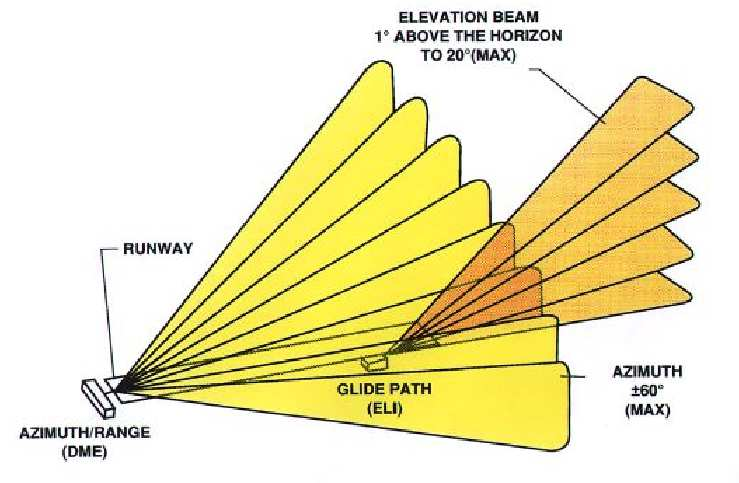
\includegraphics[height=12cm]{06.radionavegacion/Imagenes/06.Sistemas.Aproximacion/06_MLS_006.png} }
  \caption{Señales emitidas por MLS}
  \label{fig:06.MLS.seniales.emitidas}
\end{figure}


La técnica empleada en el MLS se denomina TRSB, tal como se indicó anteriormente. El equipo
de azimut emite un haz vertical en forma de abanico de dos o tres grados de ancho, que barre el
espacio horizontalmente con movimiento de ida y vuelta.

En el momento en que el haz intercepta al avión, se produce la emisión de una señal que activa un
contador, mientras que el haz sigue barriendo hasta llegar al final, cuyo tiempo es conocido. Después
vuelve, hasta que detecta de nuevo a la aeronave, momento en el cual envía otra señal que detien al
contador. El tiempo transcurrido es proporcional al ángulo que forma la trayectoria seguida por el
avión con el eje.

El barrido se divide en dos búsquedas:

\begin{description}
     \item[\bf TO]  Travel Order
     \item[\bf FRO] Flexible Response Option
\end{description}

Denominando $T_0$ al tiempo transcurrido entre dos pasadas consecutivas del haz por el eje y $\omega$ a
la velocidad angular del haz, el ángulo de situación de la aeronave se deduce directamente:

\[ \displaystyle \theta = \frac{T_0 - t}{2}\,\omega
  \]

Para comprender mejor el funcionamiento del equipo, se analizan tres casos posibles de situación
de la aeronave:


\begin{itemize}
\item \textbf{Caso 1:} $t < T_0\Longrightarrow \theta < 0$, por lo cual la aeronave se encuentra a
  la derecha.  
\item \textbf{Caso 2:} $ t = T_0 \Longrightarrow \theta = 0$, por lo cual la aeronave se
  encuentra en el centro.


\item \textbf{Caso 3:} $ t > T_0 \Longrightarrow \theta > 0$, por lo cual la aeronave se encuentra a la izquierda.
\end{itemize}


\begin{figure}[!htb]
  \centering
  {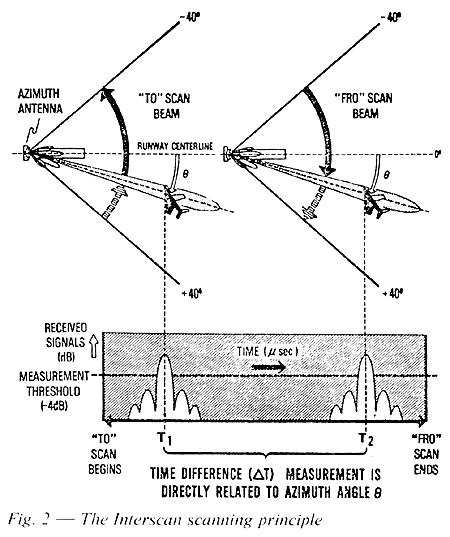
\includegraphics[width = 0.75\textwidth]{06.radionavegacion/Imagenes/06.Sistemas.Aproximacion/06_MLS_007.png} }
  \caption{Técnica de barrido del MLS}
  \label{fig:06.MLS.tecnica.barrido}
\end{figure}



El equipo de elevación radia un haz horizontal, también con forma de abanico, pero que barre el
espacio de forma vertical.

El MLS amplía la cobertura de sus haces con respecto al sistema ILS. El barrido en los sectores
de entrada o frontal y de salida o trasero es diferente.

\begin{figure}[!htb]
  \centering
  {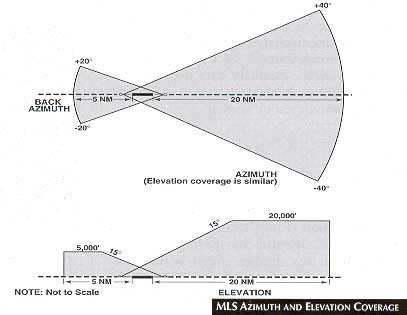
\includegraphics[width = 0.75\textwidth]{06.radionavegacion/Imagenes/06.Sistemas.Aproximacion/06_MLS_008.png} }
  \caption{Cobertura de las señales del MLS}
  \label{fig:06.MLS.cobertura.seniales}
\end{figure}

\begin{description}
\item[\bf Sector frontal]  forma un abanico que se
  extiende en azimut hasta 40º a cada lado de la pista.  En elevación
  cubre entre 0º y 15º de pendiente. Alcanza hasta 20 millas náuticas
  ( = 37 km) desde el umbral de pista y la elevación llega a los 20000
  pies (6000 m).


\item [\bf Sector trasero] en acimut sólo se extiende 20o a cada lado, con una pendiente de 0o a 15o . Su
alcance llega hasta 5 millas náuticas (9,26 km) desde el umbral de pista, con una altitud de
5000 pies (1500 m).

Se puede representar el diagrama de radiación desde una vista en planta, según la Figura \ref{fig:06.MLS.cobertura.seniales}.


\subsubsection{Ventajas y desventajas del MLS}
\label{sec:06.MLS.ventajas+desventajas}

Se considera al MLS tecnológicamente más avanzado que el ILS, al superar varias de sus deficiencias y proporcionar más seguridad. Pero también posee serie de ventajas y desventajas, las cuales se
presentan en la Tabla 1.
\end{description}

\begin{landscape}
  \begin{table}[!htb]
    \centering
    \caption{Ventajas y desventajas del MLS}
    \label{tab:06.MLS.ventajas+desventajas}

    \begin{tabular}{m{0.45\linewidth}m{0.45\linewidth}}
\rowcolor{cyan!40}
      {\bf Ventajas}  & {\bf Desventajas}  \\  \hline

      \begin{itemize}
      \item Poca importancia por el terreno. El diagrama de radiación
        se ve menos afectado.
        
\item Utilización por cualquier tipo de aeronave, incluso helicópteros.

\item       Mayor número de canales. Tiene 200 canales separados 300
MHz, en comparación con los 40 canales del ILS.

\item No interfiere en FM. Las emisiones de FM no deterioran la
información, ya que la frecuencia de trabajo es elevada, del
orden de 5 GHz.

\item Áreas críticas y sensibles reducidas. Todo ello es debido a la
utilización de microondas.

\item       Múltiples trayectorias. Las proporciona tanto en ángulo de
descenso como en desviación respecto al eje de la pista.
      
\item Instalable en cualquier aeropuerto. El ILS no se puede instalar en zonas montañosas y abruptas.

\item       Transición entre radioayudas. El sistema MLS presenta una
mayor flexibilidad.

\item Información de aproximación frustrada. El equipo de azimut
posterior proporciona información de guiado en la maniobra
de salida frustrada.
\end{itemize}

&
      \begin{itemize}
        
      \item Necesita mayor número de antenas a bordo que
el ILS.

\item La lluvia provoca serias atenuaciones de las
señales a tan alta frecuencia

\item  Los equipos componentes son muy costosos.

\item Las compañías privadas son reticentes a sustituirlo en sus flotas porque el equipo de a bordo
es más caro que el del ILS.

\item La aparición de los sistemas de navegación por
satélite cuestionan su implantación, ya que la
precisión que proporcionan va en aumento.

\end{itemize}
   \\ \hline
    \end{tabular}
  \end{table}
\end{landscape}


















